\documentclass[10pt]{article}
\usepackage[utf8]{inputenc}

\title{Distribution and Optimization of Electric Vehicle (EV) Charging Stations}
% \author{$\mathbf{IMMC18865802^\#}$}
\author{
\textbf{IMMC Team }$\mathbf{IMMC18865802^\#}$\\
Ruochuan ``Steven" Liu, Jiarui ``Jerry" Shan, Tianyu ``Wendy" Zhang, Yutong Zhang\footnote{Names of the authors are arranged by ascending lexicographic order.}
}
\date{February 6, 2018}
\usepackage[usenames]{color} %used for font color
\usepackage{amssymb} %maths
\usepackage{amsmath} %maths
\usepackage[a4paper, total={7.05in, 10.1in}]{geometry}
\usepackage{fancyhdr}
\usepackage[parfill]{parskip}
\setlength{\parindent}{2em}
\setlength{\lineskip}{10pt}
\usepackage{indentfirst}
\definecolor{linkblue}{RGB}{50,100,230}
\usepackage[colorlinks=true, linkcolor=linkblue, urlcolor=linkblue, bookmarks=true, linktoc=none]{hyperref}
% \pagestyle{empty}
% \usepackage{booktabs}
\usepackage{graphicx}
\usepackage{tabularx}
\usepackage{multirow}
\usepackage{polyglossia}
\usepackage{gensymb}
\usepackage{appendix}
\usepackage{lmodern}
\usepackage{mmacells}
\usepackage{minted}

\mmaDefineMathReplacement[≤]{<=}{\leq}
\mmaDefineMathReplacement[≥]{>=}{\geq}
\mmaDefineMathReplacement[≠]{!=}{\neq}
\mmaDefineMathReplacement[→]{->}{\to}[2]
\mmaDefineMathReplacement[⧴]{:>}{:\hspace{-.2em}\to}[2]
\mmaDefineMathReplacement{∉}{\notin}
\mmaDefineMathReplacement{∞}{\infty}
\mmaDefineMathReplacement{��}{\mathbbm{d}}

\mmaSet{
  morefv={gobble=2},
  linklocaluri=mma/symbol/definition:#1,
  morecellgraphics={yoffset=1.9ex}
}

\newcommand\bigfrown[2][\textstyle]{\ensuremath{%
  \array[b]{c}\text{\resizebox{6ex}{.7ex}{$#1\frown$}}\\[-1.3ex]#1#2\endarray}}

\begin{document}
\maketitle
\part{Summary \& Keywords}

Following the emergence and growth of the electric vehicle (EV) industry and the pressure of environmental protection, it becomes urgent to promote the use of EV to reduce air pollution caused by tail-gas. A major restriction of this goal is that charging stations and related infrastructures are often underdeveloped. In section 2, we propose a solution to optimize the locations for charging stations given the locations of EV users using a range of techniques, including a probability mass function $P$ that estimates the probability that EV users would go to each of the available charging station, an algorithm that establishes a continuous bijection between the coordinate system given in the problem and the longitude and latitude of each point, and an algorithm that uses an online map API to calculate the length of the shortest routes between two points.

In order to solve the location selection problem, a proper and well-defined metric must be established for the estimation and optimization of the cost. Clearly, the coordinate system and Euclidean metric provided along with the coordinates of the demand and candidate locations (and the map itself) are not suitable, since the Earth is a quasi-spherical astronomical object. In the article the formula calculating the great-circle distance is deduced and explained, and the deviation analysis of two metrics is carried out.

Moreover, it is clear (as stated below) that the EVs must be driven along pre-existing roads instead of a direct great-circle path from one point on the sphere to another, thus the article incorporates the LBS (Location-Based Service) in order to access the driving path and duration data in real time from the Internet. The LBS providers chosen are Google Map and Gaode Map (Alibaba AMap), and the programs used to request for data from the LBS are appended in the appendix.

The article models the behavior of EV users with high accuracy regarding their selection preference of multiple charging stations by defining a probability mass function, considering that exogenous factors other than distance often play a role in EV users' decision-making. To do so, real-world data has been evaluated from a survey that was conducted for the purpose of this paper.

Computer software and computational methods are taken advantage of in the paper to perform calculations involving large volumes of data, including programs in 

Multiple models aiming to optimize choices which a charging station company or government institution could make are discussed. In particular, microeconomics analyses, Lagrangian multiplier and partial differentiation served as informative tools that would benefit both EV users and charging stations while considering the social welfare of the city's economy. Relevant implications are elaborated in the last section from a variety of perspectives.

\textbf{Keywords: Planetary Cartography, Spherical Geometry, Mercator Projection, Spherical Distance, Location-Based Service, Multivariate Constrained Optimization, Lagrangian Optimization with Inequality Constraints, Discrete Probabilistic Distribution, Continuous Probabilistic Distribution, Exponential Decay Model}

\newpage
\tableofcontents

\pagestyle{fancy}
\fancyhf{}
\rhead{IMMC 18865802}
\lhead{Page \thepage}

\newpage
\part{Solution Paper}
\section{Introduction}
\subsection{Restatement of the Question}
This question delineated three tasks: 
\begin{enumerate}
    \item Construct a model for selecting the location and level of charging stations by considering both the initial construction cost of charging stations and minimization of charging cost for EV users. Then use our model to determine the location and level for each charging station and the distribution characteristics of EV users on choosing charging station at each demand location.
    \item Create a model to plan and adjust the charging price based on periods of time-of-use for stations of fast-charging mode and with rechargeable power batteries, aiming to minimize the cost for charging stations to purchase general industrial electricity, with considering of behavior such as charging price, distribution of EVs charging during a whole day, etc. 
    \item From different perspectives (such as technological, commercial, or public policy perspectives), analyze the problems impeding the broad application of charging piles/stations and give our solution proposal.
\end{enumerate}

\subsection{Assumptions}
\begin{enumerate}
\item 
The electric energy used to charge each car is the same;
\item 
All drivers are rational and know the location of every charging station;
\item 
All EV users and their vehicles are homogeneous, and they have the same level of wealth, and that the charging stations are aware of this fact;
\item 
Once constructed, charging stations do not incur maintenance fees;
\item 
Drivers behave according to their self-interest, and always choose the charging station which they believe is the optimal choice;
\item EV users travel back to their demand points after charging their vehicles;
\item The pricing of every charging station is identical;
\item The charging behavior of EV users can be influenced by incentives (e.g. price at peak and valley hours), and that EV users always know the price of charging their vehicles at specific time ranges;
\item All EV users assume that there would always be an outlet available at a charging station and they would be able to charge their EV whenever they park;
\item The vertical and horizontal markings on the map are parallel to the earth's longitudes and latitudes, while the distance between parallel markings is not proportional to the distance between the earth's longitude and latitude, in other words, the map is charted with a variant of the Mercator Projection Method; 
\item The demand for one recharge mode is independent from that of another.(i.e. EV users already decided how they would like to recharge their vehicles before they arrive, and would queue for their respective recharging slots); and
\item The amount of EVs remain constant over time.
\end{enumerate}
\newpage
\subsection{Notations}
{\renewcommand{\arraystretch}{1.9}%
\label{Definitions}
\begin{table}[htbp]
\label{tabular:defini}
    \centering
    \begin{tabularx}{6in}{c|c|X}

        Symbol & Symbol Name & Definitions \\
        \hline
        
        \multirow{2.5}{*}{\centering $D$} &
        \multirow{2.5}{*}{\centering Demand Point} &
        \small{As used in the problem description, a demand point is a 2-D coordinate that represents the location of a certain number of EV users who demand a recharge of their vehicles.} \\
        
        \hline
        
        \multirow{2}{*}{\centering $C$} &
        \multirow{2}{*}{\centering Construction Cost} &
        \small{Represents the construction cost of a particular solution (selection of candidate points). Used when analyzing long-term cost trends.} \\
        
        % \hline
        
        % \multirow{4}{*}{\centering $\upsilon$} &
        % \multirow{4}{*}{\centering Unit Scaling Factor} &
        % \small{A constant representing the ratio between 1km and one unit used in the coordinate system provided in the statistics tables and the map. In our paper, we have shown that $\upsilon \approx 0.013576.$} \\
        
        \hline
        
        \multirow{6}{*}{\centering $\gamma$} & \multirow{6}{*}{\centering Distance Selection Bias} &
        \small{This number defines how sensitive EV users are when considering charging stations of different distances from them. $\gamma = \log_r(2)$, where $r$ is the constant of proportionality defined as follows: if two charging stations $S_1$ and $S_2$ are $x$ and $rx$ kilometers away from a demand point $D$ respectively, then an EV user at $P$ is twice as likely to visit $S_1$ to charge than $S_2$.} \\
        
        \hline
        
        \multirow{3}{*}{\centering $y(t)$} &
        \multirow{3}{*}{\centering Linear Cost Function} &
        \small{A function of the form $Ct + b$ that estimates the total cost of the society over time. The aim of question 1 is to minimize its value.}\\
        
        \hline
        
        \multirow{1.5}{*}{\centering $S$} &
        \multirow{1.5}{*}{\centering Charging Station} &
        \small{In this article, capital $S$ denotes the coordinates of charging stations.}\\
        
        \hline
        
        \multirow{2}{*}{\centering $\xi(x,y)$} &
        \multirow{2}{*}{\centering Longitude-Latitude Conversion Function} &
        \small{maps the planar rectangualar coordinate to the longitude-latitude coordinate of Earth.}\\
        
        \hline
        
        \multirow{3}{*}{\centering $\psi(r,\lambda_1,\phi_1,\lambda_2,\phi_2)$} &
        \multirow{3}{*}{\centering Spherical Distance Function} &
        \small{calculates the spherical distance, the length of the shortest link on the surface of the sphere between two points thereon.}\\
        
        \hline

    \end{tabularx}
    \caption{Symbols and Definitions}
    \label{tab:definitions}
\end{table}}

\section{Location Selection for Charging Stations}
\subsection{Objectives Breakdown}
In order to determine the optimal locations and levels for the charging stations, we will first define the stardard which we will use to evaluate the effectiveness of a possible solution to the given problem. Before all, the priority is to ensure that all users can find a station to charge, and the locations of charging station should be chosen so that EV users can always charge at the station of their first choice if they behave in a way that is similar to that of our model. The intuitive justification of this primary objective is that the cost for EV users would increase significantly if they have to search for an alternative charging station after arriving at the first (unavailable) station, provided that they have no prior knowledge of the stations' availability. Moreover, the need for EV users to visit two stations and the fact that spare service capacity is available at the second station are indicative of an inefficient solution where resources are misallocated. Thus, we believe that an efficacious solution is one which takes the experience and travel expenses of EV users into account.

Next, the construction cost should be considered. It is explicitly stated in the problem that both \textsl{“the initial construction cost of charging station”} and \textsl{“the charging cost for EV users”} should be considered. This naturally leads to a question: while it is apparent that there exists a trade-off between the two costs, which one should be prioritized? How should we balance between the two?

It turned out that both costs are equally important to reduce, since, from an economics perspective, the city's most efficient allocation of resources relies on minimal total (society) expenditure. However, because the construction cost is a one-time expenditure, it suggests that in order to compare two solutions, we must take long-term expenditure into account. Assuming that the total charging cost ($C$) of the EV users in the city is constant on any given day, we could model the accumulative cost ($y$) of a solution with initial construction cost $b$ as
\begin{equation}\label{eq:1}
y(t) = Ct + b,
\end{equation}
where $t$ is the number of days after the initial construction, equivalent to the expected total number of kilometers that the EV user in this city will travel per day to arrive at the charging station of their choice. A long-term optimal solution will be one which minimizes $C$, since it delivers the greatest benefit to EV users.

\subsection{Behavior of a Typical Consumer}\label{behavior}
While EV users are assumed to be rational and are fully aware of the distance from their demand locations to the charging stations nearby, any modeling of a system that involves human behavior is likely to involve uncertainty in predicting individuals' choices. Consequently, a stochastic model that could account for variables in the system is highly preferred. In the case of charging station preference, there are numerous reasons to assume that an individual EV user at a given demand point does not always visit the same charging station, as they would gain more utility by visiting an alternative station. Two of such reasons are given below:
\begin{enumerate}
    \item The EV user plans to go to a particular destination on that day, and chooses a charging station that is along that route (between his demand location and his destination).
    \item Due to traffic congestion, a EV user resorts to another charging station (likely the second-closest station) on that day.
\end{enumerate}
To account for these unlikely but possible circumstances, we construct a discrete probability density function that determines the likelihood for an EV user at a given demand point $D$ to visit a particular charging station $S_i$ from a choice of $1 \leq n \leq 10$ available charging stations $S_1 \dots S_n$: 
\begin{equation}\label{eq:2}
P\left(D, S_i, \gamma\right) = \frac{d\left(D, S_i\right)^{-\gamma}}{\displaystyle\sum_{k=1}^n d\left(D, S_k\right)^{-\gamma}},
\end{equation}
where $d$ is a suitable distance function for two points on a map, which will be determined later in this article. $\gamma$ is the estimated \textbf{distance selection bias} of EV users, which is established as $\log_{1.1}(2) \approx 7.27254$ from the data of 21 adult driver's preferences. (See Appendix \ref{survey}) Informally, $\gamma,$  a positive real number, indicates the importance of distance as a factor in the average EV user's decision-making for selecting a charging station. $\gamma \to \infty$ implies that EV users will \textsl{always} choose the closest station, and $\gamma \to 0$ implies that EV users have \textsl{absolutely} no preference in choosing one charging station or another due to distance differences. This ensures that an EV user's probability of choosing a particular charging station tends to 0 as their distance to that station tends to positive infinity, and tends to 1 as this distance tends to 0.

A notable issue with this probability is that it is undefined when either $D = S_i$ in the numerator or $D = S_k$ in the denominator. This is because $d\left(D, S_i\right) = 0$, and $0^{-\gamma} = \frac{1}{0^\gamma}$. Yet, $P(D,S_i,\gamma)$ is valid when $D \notin \{S_1 \dots S_n\}$. To avoid division by zero, we rewrite $P$ in the form of a limit.

\begin{equation}\label{eq:3}
P\left(D, S_i, \gamma\right) = \lim_{m \to 0} \frac{\left[ d\left(D, S_i\right) + m \right]^{-\gamma}} {\displaystyle\sum_{k=1}^n \left[d\left(D, S_k\right) + m \right]^{-\gamma}}
\end{equation}

At $D = S_i$, the limit becomes
\begin{equation} \lim_{m \to 0} \frac{\displaystyle\frac{1}{m^\gamma}}{\displaystyle \sum_{k=1}^{i-1} \left[d\left(D, S_k\right) + m \right]^{-\gamma} + \frac{1}{m^\gamma} + \sum_{k=i+1}^{n} \left[d\left(D, S_k\right) + m \right]^{-\gamma}} = 1,
\end{equation}
which is quite reasonable considering that EV users are extremely likely to charge their vehicles right where they are if they are in a charging station. To actually evaluate this probability mass function, we need to first determine the metric $d$, since we should not simply assume that a person can go from one location to another in a straight line.

\subsection{Longitude-Latitude Coordinate Conversion Function}
% 假设所有地图上竖线与经线平行,所有横线与纬线平行,且地图上平行的两线间的距离与其经度/纬度之差呈正比关系。
According to the assumption \_, $\xi(x,y)$ is defined with a linear relation, i.e.
\[
\xi(\overline{x})=\begin{pmatrix}1\\0\end{pmatrix}\cdot\left(k_\lambda\begin{pmatrix}1\\0\end{pmatrix}\overline{x}+b_\lambda\right)+\begin{pmatrix}0\\1\end{pmatrix}\cdot\left(k_\phi\begin{pmatrix}0\\1\end{pmatrix}\overline{x}+b_\phi\right)
\]

Based on the observation made from the map and the data from Google Map and Gaode Map, we determine that the \textbf{Demand Point 1} is on the southeast cornor of the building at \textbf{1 Wen Wu Lu, LuoMaShi, Qingyang Qu, Chengdu Shi, Sichuan Sheng, China, 610014} and the \textbf{Demand Point 9} is on the southwest cornor of the build at \textbf{18 Jin He Lu, QingYang GongShangQuan, Qingyang Qu, Chengdu Shi, Sichuan Sheng, China, 610041}, and we have located, by Google Map Geocoding API, the precise longitude-latitude coordinates of these two locations\footnote{Check the appendix for more details.}
\[
\begin{cases}
\lambda_1=104.0745339802915^\circ\\
\phi_1=30.6690810197085^\circ
\end{cases}
\quad\quad\quad
\begin{cases}
\lambda_2=104.0570672802915^\circ\\
\phi_2=30.6592861197085^\circ
\end{cases}
\]

The 4 constants $k_\lambda,b_\lambda,k_\phi,b_\phi$ is acquired by solving
\begin{align}
\begin{cases}
104.0745339802915&=\quad1268.491263 k_\lambda+b_\lambda\\
104.0570672802915&=\quad1142.110215 k_\lambda+b_\lambda\\
30.6690810197085&=\quad453.572581 k_\phi+b_\phi\\
30.6592861197085&=\quad528.465054 k_\phi+b_\phi
\end{cases}
\end{align}

Now solve and get
\[
\begin{cases}
k_\lambda=0.000138207\\
b_\lambda=103.899
\end{cases}
\quad\quad\quad
\begin{cases}
k_\phi=-0.000130786\\
b_\phi=30.7284
\end{cases}
\]

Thus
\[
\xi(\overline{x})=\begin{pmatrix}1\\0\end{pmatrix}\left(0.000138207\cdot\begin{pmatrix}1\\0\end{pmatrix}\overline{x}+103.899\right)+\begin{pmatrix}0\\1\end{pmatrix}\left(-0.000130786\cdot\begin{pmatrix}0\\1\end{pmatrix}\overline{x}+30.7284\right)
\]

Here we wish to assume that the map is generated with Mercator Projection, which means that the $\displaystyle{\begin{matrix}\mathrm{horizontal}\\\mathrm{vertical}\end{matrix}}$ coordinate grid lines on the map are parallel to the earth’s $\displaystyle{\begin{matrix}\mathrm{latitudes}\\\mathrm{longitudes}\end{matrix}}$, and the distance between each of the $\displaystyle{\begin{matrix}\mathrm{horizontal}\\\mathrm{vertical}\end{matrix}}$ coordinate grid lines is the same, while though that of each of the Earth's $\displaystyle{\begin{matrix}\mathrm{latitudes}\\\mathrm{longitudes}\end{matrix}}$ is not in order to carry out our deduction.

With this assumption in mind, we are now able to define the \textbf{great-circle distance function} as \footnote{For the construction and proof steps of this, refer to the appendix.}
\[
\psi(r,\lambda_1,\phi_1,\lambda_2,\phi_2)=2r\cdot\arcsin\left(\frac{\sqrt{2-2\sin\phi_1\sin\phi_2-2\cos\phi_2\cos\phi_1\cos(\lambda_1-\lambda_2)}}{2}\right)
\]

\subsection{Error between Mercator Projection and the Reality}
\begin{center}
\noindent\fbox{%
\parbox{14cm}{%
\begin{center}
According to Mercator projection, a cylindrical map projection that represents lines of constant course, as straight segments that conserve the angles with the meridians, the horizontal and vertical lines on the map are parallel to the  latitudes and longitudes. The map sketched by Mercator projection distorts the size of shapes as the latitude increases from the Equator to the poles, where the scale becomes infinite.
\end{center}
}%
}
\end{center}
\[
\delta(r,\lambda_1,\phi_1,\lambda_2,\phi_2)=r\left(\sqrt{(\lambda_1-\lambda_2)^2+(\phi_1-\phi_2)^2}-2\arcsin\left(\frac{\sqrt{2-2\sin\phi_1\sin\phi_2-2\cos\phi_1\cos\phi_2\cos(\lambda_1-\lambda_2)}}{2}\right)\right)
\]

\begin{gather}
A=2\pi r\cdot x\\
B=\pi\cdot x^2\\
\lim_{x\to0}\frac{A}{B}=\infty
\end{gather}
\hline
\begin{gather}
C=\Delta\lambda\cdot(2\pi r)\\
D=\Delta\lambda\cdot(2r\cdot\cos\phi\cdot\pi)\\
\lim_{x\to0}\frac{C}{D}=\infty
\end{gather}
Thus proves that the deviation of the $\displaystyle{\begin{matrix}\mathrm{area}\\\mathrm{distance}\end{matrix}}$ goes to infinity while the $\displaystyle{\begin{matrix}\mathrm{area}\\\mathrm{distance}\end{matrix}}$ itself contracts to one of the polar points.

\subsection{Real World Distance}
In previous discussions, we used the spherical distance on the surface of Earth to deduct our results for simplicity, but now we wish to consider a more realistic scenario. Obviously,
\begin{center}
\noindent\fbox{%
\parbox{10cm}{%
\begin{center}
Additional assumption: EVs can only be driven along the roads.
\end{center}
}%
}
\end{center}
holds in reality.

In order to carry our our deduction under this additional assumption, we employ the Direction \& Distance API of Gaode Map\footnote{P.S. Google Map does not provide the distance we need in Chengdu City.}\footnote{Details on the source and the acquisition of this data is recorded in the appendix, as well as the full data acquired from Gaode Map and the program requesting for them.}. Here we will provide an example for the reader's comparison: The distance between the Demand Point 1 and the Candidate Point A is 0.258228 km. However, using Gaode Map API, we obtain a distance of 0.323 km between the two points. This disparity clearly reflects the inaccuracy of calculating the distance between two points on the map using the straight distance between two points. In the rest of problem 1, we will use $d \left(x,y\right)$, as the distance function to compute the distance between two point rather than the standard Euclidean distance function.

\subsection{Distance Relations}

Now that an accurate measure of distance is established by linking with the online Gaode maps API, we can use the distance function $\mathrm{Gaode} \left(x, y\right)$ in place of $d$ to make accurate calculations that predict EV users' behavior.

We begin by consider an EV user at demand point 1 with coordinates (1268.491263, 453.572581) who makes a choice between three available charging stations A,B,C, with coordinates (1284.405914, 463.870296), (1162.705645, 593.059812), and (1158.024866,418.934812) respectively. We assume that $D$ and the candidate points are only related by distance, so the distance of each charging station to an EV user at $D$ can be reduced to an one dimension graph. By using the metric $d$, we have: $$\mathrm{Gaode}\left(D, A\right) \approx 0.323 \text{ km}, \mathrm{Gaode}\left(D,B\right) \approx 4.148 \text{ km}, \mathrm{Gaode}\left(D, C\right) \approx 2.856 \text{ km}.$$

\begin{figure}[htbp]
    \centering
    \includegraphics[width=5.5in, height=0.38in, trim=10 35 10 35]{dots.pdf}
    \caption{One-dimensional view of three charging stations relative to an EV user at point $D$.}
    \label{fig:dots}
\end{figure}

Then, using equation \eqref{eq:2}, we can distribute the total of 33 EV users to the three charging stations:

{\renewcommand{\arraystretch}{1.9}%
\begin{table}[htbp]
    \centering
    \begin{tabular}{c|c|c}
        Location & Probability & Expected EV Users (total is 33) \\
        \hline
        A & 0.999999860685 & 32.999995402594 \\
        \hline
        B & 0.000000008658 & 0.000000285702 \\
        \hline
        C & 0.000000130658 & 0.000063585013\\
    \end{tabular}
    \caption{Probability and expected demand for three charging stations relative to $D$.}
    \label{tab:dist_prob}
\end{table}}

We define the \textbf{expected distance} as the total distance of an EV user from a demand point to \underline{each} charging station multiplied by the probability that they choose that station.

In order to calculate the expected distance that an EV user at $D$ will travel to charge his vehicle, we multiply the probability of this person choosing each charging station by the distance to that station, and sum these values together: 
\begin{equation}\label{eq:3}
\mathrm{Gaode}\left(A,D\right) \cdot P(D, A, \gamma) + \mathrm{Gaode}\left(B,D\right) \cdot P(D, B, \gamma) + \mathrm{Gaode}\left(C,D\right) \cdot P(D, C, \gamma) = 0.323000364071 \text{ km}.
\end{equation}

Note that this is barely different from $\mathrm{Gaode}\left(A,D\right).$ This actually suggests that $P$ is a reasonable distribution because the stations $B$ and $C$ were arbitrarily chosen and happened to be very far from $A$, making $A$ the most likely station which the total demand at $D$ will be distributed to.


\subsection{Linear Cost Model}
Our next goal is to determine the constants $C$ and $b$ in $y(t)$ as stated in equation \eqref{eq:1}. We will first demonstrate how C could be found by getting the total distance all 996  To calculate the total expected cost of all EV users at $D$, we multiply this amount by the number of users, 33. This is the coefficient $C$ in the linear cost function \eqref{eq:1}.

Although we did not yet devise a method for computing the construction cost $b$, its effect is largely diminished as $t \to \infty$, the construction plan with the lowest long-term cost is one with minimal $C$, or the slope with the most gradual inclination. This means that all 10 candidate positions should be used as charging positions to minimize long-run daily expense for EV users (which would also minimize the society's costs). Let this minimal cost be $C_\text{min}$. By extending equation \eqref{eq:3} to $D_1 \dots D_{30}$ and $S_1 \dots S_{10}$, we have
\begin{equation}\label{eq:4}
C_\text{min} = \sum_{i=1}^{30}\sum_{j=1}^{10}d\left(S_j, D_i\right) \cdot P(D, S_j, \gamma) = 57.104452532397 = \text{¥} 164.643936.
\end{equation}

Note that we multiplied the cost by 2 because we assume that the EV users will return to their demand points after charging their vehicles.

Finally, to complete the optimal cost function $y_\text{opt}(t)$, we must find $b$. For each charging station, we sum the total expected EV users from every demand point, and choose the smallest charging station level such that the service capacity is greater or equal to that number.\newline

{\renewcommand{\arraystretch}{1.9}%
\begin{table}[htbp]
    \centering
    \begin{tabular}{c|c|c}
        Location & Expected EV Users (total is 996) & Initial Construction Cost (¥) \\
        \hline
        $S_1$ & 94.611483449091 & 400,0000 \\
        \hline
        $S_2$ & 214.65988063449 & 530,0000 \\
        \hline
        $S_3$ & 71.315730731205 & 400,0000 \\
        \hline
        $S_4$ & 101.28173137436 & 400,0000 \\
        \hline
        $S_5$ & 57.072296517926 & 350,0000 \\
        \hline
        $S_6$ & 76.838476260734 & 400,0000 \\
        \hline
        $S_7$ & 161.39618857301 & 530,0000 \\
        \hline
        $S_8$ & 81.059158774683 & 400,0000 \\
        \hline
        $S_9$ & 58.629298428917 & 400,0000 \\
        \hline
        $S_{10}$ & 79.135755255593 & 400,0000
    \end{tabular}
    \caption{Expected daily visits by station and estimated construction cost.\newline}
    \label{tab:dist_cost}
\end{table}}

The total initial construction cost for the 10 stations is therefore 4240,0000. An advantage of this solution is that most stations have some spare capacity, so if one station is accidentally down for maintenance or receives more charging requests in a day than the expected amount, then the charging stations would still satisfy the charging requests from all of its customers. Our model is now complete: $$y_\text{opt}(t) = 1815.625858t + 42400000.$$

While 4240,0000 is certainly not the minimal construction cost, reducing this cost will result in a greater coefficient for $t$ in the linear cost function, which could result in a higher economic cost in the long-run. It is possible that the government has a limited budget for the initial construction cost, and is unable to afford this amount. If that's the case, another plan is needed. To demonstrate this expenditure constraint, consider that the government wants to minimize the construction cost, or $b$ in the linear cost function.

First, referring to table 3 in the problem's appendix, it is evident that the construction per unit of service decreases as the service capacity increases. This indicates that a way to minimize the initial construction cost is to only build 3 charging stations, each with level 1 service capacity (350 per day), given that none of the stations is expected to receive a daily demand that is greater than 350. This is theoretically possible as $3 \times 350 = 1050, and 1050 > 996.$ Therefore, minimal construction cost $b = 3 \times \text{¥}650,0000 = \text{¥}195,0000.$ The question is, how do we determine which 3 candidate positions to use? If the charging station locations are chosen inappropriately, then the 996 total EV users will not be distributed evenly among these three stations according to our probability distribution model, resulting in one or two stations that exceed their service capacity. For example, if we arbitrarily choose candidates B, C, and J at coordinates (1162.705645,593.059812), (1158.024866,418.934812) and (920.241263,427.360215) as the three charging stations, the expected distribution of EV users arriving at these stations is demonstrated in Table \ref{tab:dist_bad_example}. 

{\renewcommand{\arraystretch}{1.9}%
\begin{table}[htbp]
    \centering
    \begin{tabular}{c|c}
        Station Location & Expected EV Users Arriving Per Day \\
        \hline
        B & 266.87907066901 \\
        \hline
        C & 148.25016520819 \\
        \hline
        J & 580.87076412280\\
    \end{tabular}
    \caption{EV user demand distribution for stations B, C, and J.}
    \label{tab:dist_bad_example}
\end{table}}

Apparently, considering that charging station J would receive much more demand from EV users than the electricity it can provide, this construction plan is an unsuccessful one.

Due to the large number of possible combinations for choosing three charging stations, it is unrealistic to calculate the demand distribution for each of these selections. In fact, the number of unique combinations of threes that can be made from 10 candidate locations is $$\mathrm{C}_{10}^3 = \frac{10!}{(10-3)!\cdot 3!} = 120.$$

To speed up the method for determine the three optimal candidate locations, we devised a computer algorithm that uses two criteria against each combination:
\begin{enumerate}
    \item The expected number of EV users for each station must be within the service capacity, 350.
    \item The expected distance that EV users around the city will travel to these three charging stations is kept minimal.
\end{enumerate}

Unfortunately, it turned out that there is no combination of 3 stations that would make sure none exceeds the highest service capacity (350), so we moved on to combinations of 4 stations. The total number of trials is given by $$\mathrm{C}_{10}^4 = \frac{10!}{(10-4)!\cdot 4!} = 210.$$
The stations that matched these criteria are D, E, I, and J. By mapping the expected visits for each of these stations with the lowest station level that has a service capacity higher than this estimation, we have $b = \text{¥}2230,0000$. The program also gives $C = 2 \cdot  4226.827881$ km. Note that we multiplied the Gaode distance by 2 because we assume that the EV users would travel the same distance to return to their demand points. We now have the linear cost function for minimal construction cost: \begin{equation}
y_\text{init}(t)=8453.655762t + 22300000.
\end{equation}

{\renewcommand{\arraystretch}{1.9}%
\begin{table}[htbp]
    \centering
    \begin{tabular}{c|c|c}
        Station Location & Expected EV Users Arriving Per Day & Expected Total Travelling Distance \\
        \hline
        D & 247.14371025221 & 1040.1699044398 \text{ km} \\
        \hline
        E & 315.16803414765 & 1339.1636311168 \text{ km} \\
        \hline
        I & 93.03553234521 & 373.93089021132 \text{ km} \\
        \hline
        J & 340.6527232549 & 1473.5634560703 \text{ km}
    \end{tabular}
    \caption{EV user demand distribution for optimal stations (D, E, I, J).}
    \label{tab:dist_good_example}
\end{table}}

\begin{figure}[htbp]
    \centering
    \includegraphics[scale=.62,trim=45pt 0 0 0,clip]{linear_plot.pdf}
    \caption{Economic-wise and user-wise linear cost functions}
    \label{fig:opt_lcf}
\end{figure}

Figure \ref{fig:opt_lcf} again suggests that there is a trade-off between short-term and long-term cost reduction. Any other possible construction plan would result in a linear cost function between the two curves in Figure \ref{fig:opt_lcf} in the sense that $1815.625858 \le C \le 8453.655762$ and $22300000 \le b \le 42400000$. Depending on the priority of the city's economy and the budge available, the government may adopt any scheme in this range.

\section{Time-of-use Pricing}

The net cost of a charging station is largely determined by its expense and revenue. In this section, we will develop models that propose ways to optimize the price that should be set for EV users during each time interval that minimize the cost for charging stations to purchase general industrial electricity. One method is to maximize the profit which the charging station can earn from its customers by choosing the appropriate prices to charge. For each of the three recharging modes (slow-charging mode, fast-charging mode, and battery swapping mode), we will find the price which maximizes customer satisfaction by balancing the number of customers with the efficiency of the station, assuming that the station's efficiency is determined by infrastructural constraints which are fixed.

A well-developed model on the handling of customers in a service system is the \texstbf{M/M/s queuing model}, which finds the equilibrium point between service rate and arrival rate per hour through the \textbf{steady-state distribution}. The model assumes that the system's total buffer (service capacity + queuing capacity) is infinite and that the queuing policy is \emph{first-come-first-serve}. Additionally, all servers are assumed to be identical and operate independently. This model will be used to calculate the optimal price of charging which a charging station should set, based on the demand from EV users. In our scenario, let each server be a charging slot (battery-swapping stations will be discussed in a separate model), and suppose that a charging station has $s$ slots that can operate simultaneously, each with service rate $\mu$. Then, given that there are $n$ customers in the service system, the total service speed is given by $n\mu$ when $n\le s$ and $s\mu$ when $n \ge s$.

Let $\eta$ be the mean of a Poisson process that models the arrival rate of EV users per hour. At any $n \in \{0\} \cup \mathbb{N}$, let $P_n$ denote the probability that there are $n$ customers in the station. This permits us to associate the probability that there are $k$ customers in the system with that of $k-1$ customers:
$$P_1 = \frac{\eta}{\mu}P_0$$
$$P_2 = \frac{\eta}{2\mu}P_1$$
$$\vdots$$
$$P_k = \frac{\eta}{n\mu}P_{k-1}, k \le s$$
$$P_k = \frac{\eta}{s\mu}P_{k-1}, k > s.$$

Note that $P_0 > 0$, because we expect that queues are finite and are temporary at the gas stations. It is not difficult to see that each $P_k$ with $k > 1$ can be represented as a function involving $P_0.$

\begin{equation}
    P_k = \begin{cases}
    \displaystyle\frac{\eta^k}{k!\mu^k}P_0 \  & k \le s \\[9pt]
    \displaystyle\frac{\eta^k}{k! \mu^k s^{k-s}}P_0\ & k > s.\\
    \end{cases}
\end{equation}

Since $\sum_{i=1}^\infty P_i = 1$, we can further compute $P_0$:

\begin{equation}
    P_0\left(\sum_{i=0}^s \frac{\eta^i}{i!\mu^i} + \sum_{j=s+1}^{\infty} \frac{\eta^j}{s! \mu^j s^{j-s}} \right) = 1.
\end{equation}
\begin{equation}
    P_0 = \left(\underbrace{\sum_{i=0}^s \frac{\eta^i}{i!\mu^i}}_{\text{finite terms}} + \underbrace{\frac{s^s}{s!}\cdot \sum_{j=s+1}^{\infty} \left(\frac{\eta}{\mu s}
    \right)^j}_{\text{infinite series}} \right)^{-1}
\end{equation}

Because $P_0 > 0$ as previously justified, the infinite (geometric) series must converge. This requires that the common ratio $\frac{\eta}{\mu s} < 1.$ This is known as the \textbf{steady state condition}. When the arrival rate ($\eta$) and service rate ($\mu$) are known for a given time-of-use period, it becomes possible to determine the probability that the station is empty during that period. Furthermore, we can calculate the expected (average) number ($E(n)$) of customers at the charging station.

The method of finding $E(n)$ is similar to that of a continuous random variable. When calculating the expected value $E(X)$ of a continuous random variable $X$ given by a probability density function $f: [a,b] \to \mathbb{R}^+$, we evaluate the following integral:
\begin{equation}
    E(X) = \int_b^a x f\left(x\right) dx.
\end{equation}
Likewise,
\begin{align}
    E(n) & = \sum_{n=0}^\infty n \cdot P_n \\
    & = \sum_{n=0}^s n \cdot P_n + \sum_{n=s+1}^\infty n \cdot P_n \\
    & = \sum_{n=0}^{s}\frac{\eta^n}{n!\mu^n}P_0 + \sum_{n=s+1}^\infty \frac{\eta^n}{n! \mu^n s^{n-s}}P_0.\label{eq:5}
\end{align}

When $\eta,\mu$ and $s$ are given, $P_0$ can be computed, and plugging in these four values into equation \eqref{eq:5}, we get $E(n)$. This estimation serves as a useful indicator for whether the charging station has too many customers, or too few customers, which allows it to adjust as needed. Oftentimes, $E(n)$ should be maximized but kept smaller than $s$ (number of charging slots), because while a larger arrival rate implies higher revenue per unit of time, if $E(n) > s$, the station is at risk of forming a waiting queue that not only spreads undesirable user experience, harming future reputation and arrival rate of the station, but also gives the charging station no additional revenue, since all slots are already occupied. In microeconomics, this is known as \textbf{market disequilibrium}, and indicates allocative inefficiency. According to economics theories, a market always operates best when quantity demanded perfectly meets the quantity supplied at the equilibrium price and quantity. In a given length of time $t$ at a charging station, the maximum quantity supplied is determined by $\mu t$, and the quantity demanded is $\eta t$. More specifically, since we cannot assume the arrival rate to be the same at peak hours, flat hours and valley hours, we denote the expected quantity demanded during each of these 3 time-of-use periods in a 24-hour period by $\eta_p t, \eta_f t$, and $\eta_v t$. In the rest of this article, $\eta$ without subscript is used to refer to all 3 aforementioned values.

$\eta$ is responsible for maximizing profit, since a charging station only gains revenue if it has customers. $\eta$ is determined by a variety of factors, such as time of day, charging price at the station, charging price of other (alternative) charging stations nearby, types of recharging mode available at the station, etc. To simplify our model, we will view $\eta$ as a monotonically decreasing function of a single variable $x$ (this is similar to the demand curve function used in microeconomics models), which represents the price per kilowatt hour offered to EV users at the station. As the price increases, the arrival rate decreases. All other factors associated with $\eta$ are assumed to be held constant.According to research, the \textbf{price elasticity of demand} for electricity is approximately constant at $-0.32$ for all time-of-uses, which is equivalent to the gradient of $\eta_p(x) \cdot t_p,\eta_f(x) \cdot t_f$ and $\eta_v(x) \cdot t_v$, where each time coefficient denotes the length of each time-of-use. $\eta_p(x)\cdot t_p$ is then $$\int -0.32\, dx = -0.32x + c_p,$$ where $c_p$ is a constant that needs to be determined for the charging station of interest. Similarly, we have $$\eta_f(x) \cdot t = -0.32x + c_f \text{\  and \ } \eta_v(x) \cdot t = 0.32x + c_v.$$ For demonstrative purposes, consider a particular charging station with $c_p = 150$.


For each time period (peak hours, flat hours or valley hours), the expected profit gained in the designated time period is given by the difference in the total revenue and total cost, multiplied by the number of customers. For instance, during the peak hours of a typical day, the expected profit is $$\rho = n(x_p - 1.322),$$ where 1.322 is the cost of electricity during the peak hours. To maximize the profit $\rho$, both $n$ and $x_p$ need to be optimized. To do so, the most straightforward solution is to substitute one of the two variables with a function of the other. Since $n = \eta_p(x_p)$, we have
\begin{align*}
    \rho & = \eta_p(x_p)(x_p - 1.322) \\
    & = (-0.32x_p+c_p)(x_p-1.322) \\
    & = -0.32x_p^2+(0.423+c_p)x_p - 1.322c_p;\\
    \frac{dR_p}{dx_p} & = -0.64x_p+(0.423+c_p).
\end{align*}

In this particular Shanxi charging station,$$x_p = \frac{0.423+178}{0.64} = \text{¥}278.786 \text{ per kilowatt hour}.$$

This is a very large number comparing to the market price for electricity. Although theoretically setting this price would greatly benefit electricity providers, electricity is considered a necessity for people of all levels of incomes, and so its price must accommodate the poorest income earners. It is likely that the government has set a legal price floor for electricity, and makes sure that affording it is not a burden for anyone. Yet, the price cannot be too low, because it is already shown that $E(n)$ should be less than $s$, and that according to the law of demand in economics, there is an inverse relationship between the cost and the quantity demanded. This estimation of $x_p$ is also an unrealistic one, as it assumes that no other factor has influenced EV users' decision to come to the charging station, such as the relative price of alternative charging stations. Nevertheless, estimations like this one provide insight on where the optimal values are likely to be found.

Having discussed absolute pricing, it seems natural to also discuss the relative prices of electricity at three different periods of time-of-use at the charging station. We assume that there exists a dependence between the three time-of-uses in the sense that if the price for one time-of-use increases abruptly, EV users who have accustomed to this time-of-use may choose to switch to another time to charge. The ideal outcome of this optimization is to ensure that the utility rate is equally high for all three time-of-uses. In other words, all potential customers are evenly distributed in the three time-of-uses, making the best use of resources throughout 24 hours. To achieve this, we need to assume again that the only variables that can and will change are the arrival rates for the three time-of-uses. Then, we can construct a system of equations that could compute the price settings that would result in an even distribution of customers in all three time-of-uses. Let $p,f,v$ denote the percentage of EV users that are expected to charge their vehicles during the peak, flat, and valley hours. Clearly, $$p + f + v = 1,$$ and our goal is to set the prices such that $$p = f = v = \frac{1}{3}.$$ Let variables $\beta_p,\beta_f$ and $\beta_v$ each denote the price of electricity set by the charging station at each of the 3 time-of-uses, and let $$\sigma(\beta_p, \beta_f, \beta_v)$$ be a function of three variables that returns the standard deviation of $p,f$ and $v$. By doing so, we assume that it is possible to find such function. Since the only possibility that three values have 0 standard deviation is by having the same value, $\sigma$ must have an absolute minimum which has the optimal prices.

To locate this minimum, we equate $\sigma$'s gradient function with the zero vector:
\begin{equation}
    \nabla \sigma = \left<\frac{\partial \sigma}{\partial \beta_p},\frac{\partial \sigma}{\partial \beta_f},\frac{\partial \sigma}{\partial \beta_v}\right> = \vec{0}.
\end{equation}

The case for swapping batteries is a different scenario, because different from standard and fast-charging stations, a charging station that supports battery swapping can make an additional decision of when to recharge the depleted batteries to minimize cost. Ideally, a charging station would prefer to have all the depleted batteries charged in the valley hours (11:00 pm to 7:00 am) or flat hours, since the price of electricity at these time-of-uses are relatively lower. The challenge, however, is to decide whether to save the batteries until then, or charge them right away. Ideally, all batteries should be charged at the valley hours, but it's unlikely to happen, as the demand for battery swapping during daytime may exceed the fully charged battery stock, and before all, the priority is to maximize the number of customers that can be served in a period of time, and if customers arrive without able to swap for a fully charged battery, then bad user experience may harm the future arrival rate of the charging station.

To optimize the timing of recharging the batteries, we should balance the total number of batteries recharged during the day with the total number of batteries that are swapped. We will also assume that battery swapping are instantaneous, since the time required to swap a battery is negligible comparing to that of recharging a depleted battery. Ideally, in valley hours, the arrival rate $\eta_v(x)$ should be less than the replenish (service) rate $R_v$, and in peak hours, the arrival rate $\eta_p(x)$ should exceed the replenish rate $R_p$. Depending on the service capacity of the station, the arrival rate $\eta_f$ may be less, greater or equal to $R_f$. (All $\eta(x)$s are functions of cost $x$) Assuming that the EV user's cost of swapping a battery is constant, the charging station could only operate if the net efficiency is non-negative: 
\begin{equation}\label{eq:inequality}
    8 (R_p - \eta_p(x)) + 8 (R_f - \eta_f(x)) + 8(R_v - \eta_v(x)) \ge 0.
\end{equation}


With this constraint, it is not difficult to see that $R_p$ should be minimized, $R_v$ should be maximized, and $R_f$ should be adjusted as needed to keep this inequality true. We also need to bear in mind that due to the infrastructural constraints of the station, none of the replenish rates can exceed the maximum rate $R_{\text{max}}$ given by $\frac{s}{T_c}$, where $s$ is the number of charging services and $T_c$ is the average time to charge one depleted battery. On the other hand, since we assume that the price of battery swapping is constant throughout the day, the three $\eta(x)$s cannot be adjusted independently, and are subject to the same cost variable $x$. Cancelling the coefficient, we can rewrite expression \eqref{eq:inequality} and $R_\text{max}$ as two distinct constraints of the system:

\begin{equation}
    R_p + R_f + R_v - \left(\eta_p(x) + \eta_f(x) + \eta_v(x)\right) \ge 0; 3R_\text{max} \ge R_p + R_f + R_v.
\end{equation}

While satisfying these constraints, a charging station should aim to maximize its profit $\rho$ by adjusting the factors which it has control over: $R_p, R_f, R_v$ and $x$. Assuming that the charging station has adjusted its supply of fully charged batteries to meet the market demand, the expected profit, or the expected output worth, of the station in a day in RMB can be given by:
\begin{equation}
    \rho =  8R_p(x - 1.322) + 8R_f(x - 0.832) + 8R_v(x - 0.369).
\end{equation}

This is a Lagrangian optimization problem with two inequality constraints. Let $\mu_1$ and $\mu_2$ be the two Lagrangian multipliers. The Lagrangian is:

\begin{align}
    L(R_p, R_f, R_v, x, \mu_1, \mu_2) =\  & 8\left[R_p(x - 1.322) + R_f(x - 0.832) + R_v(x - 0.369)\right]\\
    & - \mu_1\left[R_p + R_f + R_v - \left(\eta_p(x) + \eta_f(x) + \eta_v(x)\right)\right]\\
    & - \mu_2\left(3R_\text{max} - R_p - R_f - R_v\right).
\end{align}

When these values are known, the optimal recharge rate of depleted batteries at different time-of-uses can be known, which will reduce the total cost of the station. This is done by solving the following system of equations:
\begin{align*}
\nabla \rho & = \mu_1 \nabla \left[R_p + R_f + R_v - \left(\eta_p(x) + \eta_f(x) + \eta_v(x)\right)\right] + \mu_2 \nabla\left(3R_\text{max} - R_p - R_f - R_v\right)\\
0 & \le 3R_\text{max} - R_p - R_f - R_v\\
0 & \le R_p + R_f + R_v - \left(\eta_p(x) + \eta_f(x) + \eta_v(x)\right).
\end{align*}

Although consumers typically prefer vehicles with larger battery capacities, the performance of all batteries are limited by the laws of physics, meaning that the voltage, current (discharge rate) and quantity of electricity (charge) that remains in an EV all monotonically decrease with time as the vehicle is being used. For this reason, many electric vehicle models have hybrid engines, meaning that the vehicle can automatically switch from electric power to fuel power when electricity can no longer supply energy at a rate that meets the consumption rate. Even though hybrid vehicles are less environmental friendly comparing to their purely electrified counterparts, the unavailability of charging stations -- a major disadvantage for EV users when travelling to remote places without power stations -- is no longer a problem for hybrid vehicles as they have an alternative fuel source, and the performance of fuel does not decrease with time. Therefore, hybrid vehicles are also an effective solution to environmental pressures due to air pollution.

\section{Implications and Beyond}

While the models we presented are definitely useful in the scope of the given problem, there are many factors that must be accounted for when planning to construct charging stations in real life. Without sufficient charging stations, it would be inconvenient for EV users to charge their vehicles, which limits the popularity of new energy vehicles. This problem can be addressed differently depending on the perspective and the priorities associated with it.

\subsection{Commercial Perspective}
The commercial perspective prioritizes profitability. Inarguably, a successful charging station is one which attracts EV users, because the primary source of revenue for a charging station is the charging cost which EV users pay, and the frequency which they come could be influenced by distance of the charging station to them. For instance, if an EV driver lives very far from any charging station, they might deliberately reduce the usage of their vehicle, knowing that they have to drive for a long way to charge. Reduced (suppressed) consumption leads to reduced revenue, and that negatively impacts the aggregate demand of the economy, which is often undesirable. This is a justification of why the location of charging stations is important to EV users.

In real life, however, the candidate positions are not given. How do we determine the optimal locations for charging stations using only the demand points?

By definition, if a point $S$ is an optimal location for a charging station in a region $R$, then the total travelling distance of all demand points in $R$ to this optimal point is less or equal to that of any other point around it. Let $x$ and $y$ be two variables that represent the $x$ and $y$ coordinates of a possible charging state position, and let the total travelling distance of EV users to that point be defined by the function $D(x,y)$. Then any stationary point could be viewed as a relative extremum \footnote{A maximum or minimum.}, where first order partial derivatives $\frac{\partial D}{\partial x}$ and $\frac{\partial D}{\partial y}$ are 0. From these stationary points, we can find the optimal location or set of optimal locations with minimum total distance.

To demonstrate this optimization strategy for choosing one location for a charging station, let $R$ be a $4 \times 4$ square located at the center of a 2-D Cartesian plane. There are three demand points (with one EV user at each), $D_1, D_2,$ and $D_3$, and they are located at $(1,-1)$, $(-1,-1)$, and $(1,-1)$ respectively. The charging station must be placed within this region, with $-2 \le x \le 2$ and $-2 \le y \le 2$.

\begin{figure}[htbp]
    \centering
    \begin{minipage}[t]{0.45\textwidth}
        \centering
        \includegraphics[width=205pt,height=205pt]{dot_plot.pdf}
        \caption{\small Visualization of three demand points in $R$.}
    \end{minipage}
    \begin{minipage}[t]{0.45\textwidth}
        \centering
        \includegraphics[width=205pt,height=205pt]{density_plot.pdf}
        \caption{\small Scalar field visualization for $D(x,y).$}
    \end{minipage}
    \label{fig:density_plot}
\end{figure}

We define $D(x,y)$ as the density function, which computes the total distance of any given point $(x,y) \in R$ from the three demand points.

\begin{equation}
    D(x,y) = \sqrt{(-1-x)^2+(1-y)^2} + \sqrt{(-1-x)^2+(-1-y)^2} + \sqrt{(1-x^2)+(-1-y)^2}
\end{equation}

This allows us to construct a scalar field, as shown in figure \ref{fig:density_plot}. Purple color indicates smaller value, and the point with the deepest purple color is the stationary point – the optimal location for charging station – which we need to determine.

To determine the $x$ and $y$ coordinate of this optimal location, we first find the first order partial derivatives with respect to $x$ and $y$.
\begin{align}
\frac{\partial D}{\partial x} = -\frac{-x-1}{\sqrt{(-x-1)^2+(-y-1)^2}}-\frac{-x-1}{\sqrt{(-x-1)^2+(1-y)^2}}-\frac{1-x}{\sqrt{(1-x)^2+(-y-1)^2}},\\
\frac{\partial D}{\partial y} = -\frac{-y-1}{\sqrt{(-x-1)^2+(-y-1)^2}}-\frac{-y-1}{\sqrt{(1-x)^2+(-y-1)^2}}-\frac{1-y}{\sqrt{(-x-1)^2+(1-y)^2}}.
\end{align}

Since both of the equations evaluate to 0 only at the stationary point, we can refer to this point as $(x_0, y_0)$. Solving $$\nabla D= \left<\frac{\partial D}{\partial x}, \frac{\partial D}{\partial y}\right> = \vec{0},$$ we obtain $x_0 = y_0 = -0.577350.$ The shortest total distance is therefore $D(x_0,y_0) = 3.863703.$

We can expand this method to evaluate the optimal locations for two charging stations by having four variables: $x_1,y_1,x_2,y_2.$ To optimize four values, we will first find the total distance function $D$ and then use the same method to obtain the minimum combination.

\begin{align*}
	D(x_1,y_1,x_2,y_2) = \lim_{m\to 0} \, & \left(\frac{\sqrt{(-x_1-1)^2+(-y_1-1)^2} \left(m+\sqrt{(-x_1-1)^2+(-y_1-1)^2}\right)^{-\gamma }}{\left(m+\sqrt{(-x_1-1)^2+(-y_1-1)^2}\right)^{-\gamma}+ \left(m+\sqrt{(-x_2-1)^2+(-y_2-1)^2}\right)^{-\gamma }}\right.\\
	& + \left. \frac{\sqrt{(1-x_1)^2+(-y_1-1)^2} \left(m+\sqrt{(1-x_1)^2+(-y_1-1)^2}\right)^{-\gamma }}{\left(m+\sqrt{(1-x_1)^2+(-y_1-1)^2}\right)^{-\gamma } + \left(m+\sqrt{(1-x_2)^2+(-y_2-1)^2}\right)^{-\gamma }}\right. \\ 
	& + \left.\frac{\sqrt{(-x_1-1)^2+(1-y_1)^2} \left(m+\sqrt{(-x_1-1)^2+(1-y_1)^2}\right)^{-\gamma }}{\left(m+\sqrt{(-x_1-1)^2+(1-y_1)^2}\right)^{-\gamma }+\left(m+\sqrt{(-x_2-1)^2+(1-y_2)^2}\right)^{-\gamma }}\right. \\
	& + \left.\frac{\sqrt{(-x_2-1)^2+(-y_2-1)^2} \left(m+\sqrt{(-x_2-1)^2+(-y_2-1)^2}\right)^{-\gamma }}{\left(m+\sqrt{(-x_1-1)^2+(-y_1-1)^2}\right)^{-\gamma }+\left(m+\sqrt{(-x_2-1)^2+(-y_2-1)^2}\right)^{-\gamma }}\right. \\
	& + \left.\frac{\sqrt{(1-x_2)^2+(-y_2-1)^2} \left(m+\sqrt{(1-x_2)^2+(-y_2-1)^2}\right)^{-\gamma }}{\left(m+\sqrt{(1-x_1)^2+(-y_1-1)^2}\right)^{-\gamma }+\left(m+\sqrt{(1-x_2)^2+(-y_2-1)^2}\right)^{-\gamma }}\right.\\
	& + \left.\frac{\sqrt{(-x_2-1)^2+(1-y_2)^2} \left(m+\sqrt{(-x_2-1)^2+(1-y_2)^2}\right)^{-\gamma }}{\left(m+\sqrt{(-x_1-1)^2+(1-y_1)^2}\right)^{-\gamma }+\left(m+\sqrt{(-x_2-1)^2+(1-y_2)^2}\right)^{-\gamma }}\right).
\end{align*}

Solving
\begin{equation}
\nabla D = \left<
 \frac{\partial D}{\partial x_1},
 \frac{\partial D}{\partial y_1},
 \frac{\partial D}{\partial x_2},
 \frac{\partial D}{\partial y_2}
\right> = \vec{0},
\end{equation}

it turns out that when the candidate positions are $(-1,1)$ and $(1,-1)$, then the total distance that the three EV users are expected to travel is minimum (=2), since it is already shown that when a demand point coincides with a charging station, the distance between them is 0 and the probability of a local EV user going to that station is essentially 100\%. There is no other choice of two charging stations that would yield a total distance less than 2, because of the nature of our probability distribution model. Although it is likely to be impossible to construct a charging station right at a demand point, it makes sense to construct it as close as possible to that demand point.

With the two scenarios shown, it is not difficult to see that when optimizing the location for $k$ charging stations given $n$ demand point locations, an accumulative distance function $D$ with $2k$ number of variables is required. By equating the partial derivatives of each of these variables with respect to $D$ to 0, we can find the lowest travelling expense for EV users as well as the ideal location for the charging stations.

\subsection{Technological Perspective}

There is sufficient evidence to believe that the electric vehicle industry is growing, spurring an increasing demand in lithium ion batteries. From a technological perspective, we must consider the physical constraints of lithium-ion batteries and use this information to predict the future technological development of batteries, such as how batteries can increase their capacity.

We can model the expected discharging rate $I$ and voltage $V$ of a battery cell with time $t$ by utilizing several facts in physics:
\begin{align}
    V = IR \label{eq:v} \\ 
    P = IV \label{eq:p} \\
    -I = \frac{dQ}{dt}\label{eq:current}\\ 
    C = \frac{Q}{V} \label{eq:c}
\end{align}
where $R$ is resistance (ohms), $P$ is power (watts), $Q$ is charge (Coulombs), and $C$ is capacitance (farads). Note that $I$ is negative because the charge in the battery is monotonically decreasing over time, and we define positive current by the flow of charge out of the batter.

We hope to find an expression for $Q(t)$ which expresses the amount of charge left in a battery after $t$ seconds have elapsed, and a similar $V(t)$ which expresses voltage of the battery as a function of time.

We begin with finding a relationship between current $I$ and charge $C$. Using \eqref{eq:v}, \eqref{eq:current} and \eqref{eq:c}, we have

\begin{equation}
    -I = \frac{d Q}{d t} = -\frac{V}{R} = -\frac{Q}{RC}.
\end{equation}

Since $\tau = \displaystyle\frac{Q}{RC}$ is a constant, we can solve the differential equation by separating variables $t$ and $Q$:
\begin{align}
    \int \frac{dQ}{Q} & = \int-\frac{dt}{\tau} \\
    \ln (Q) & = e^{-\frac{t}{\tau} + c} \\
    \therefore Q(t) & = Q_0 e^{-\frac{t}{\tau}}
\end{align}
Similarly, the voltage of a battery can be modelled by solving another set of differential equations by utilizing \eqref{eq:c}.
\begin{align}
    \Delta Q & = C \Delta V,\\
    I = \frac{V}{R} & = \frac{dQ}{dt} = C\frac{dV}{dt},\\
    C\int \frac{dV}{V} & = \int R\, dQ,\\
    \ln (V) & = -\frac{t}{RC} + c \\
    \therefore V(t) & = V_0 e^{-\frac{t}{\tau}}.
\end{align}

At any time, the energy stored in a capacitor can be expressed as a function of capacitance and charge. Since the definition of \textbf{1 volt} is the potential difference at which a charge of 1 Coulomb gains 1 Joule of energy, $V$ represents energy per unit charge, and can be expressed in the equation
\begin{equation}
    \Delta E = V \cdot \Delta Q.
\end{equation}

Substituting $V$ with $\frac{Q}{C}$, and taking the integral on both sides, we have
\begin{equation}\label{eq:energy}
    \int dE = \int \frac{Q}{C}\, dQ = \frac{1}{2}\frac{Q^2}{C} = \frac{1}{2}CV^2.
\end{equation}

Using a similar method, we can also deduce that $I(t) = I_0 e^{-\frac{t}{\tau}}$. For illustrative purpose, a graph showing the exponential growth rate for the voltage of a typical electric vehicle battery is shown in figure \ref{fig:velocity}.
\begin{figure}
    \centering
    \includegraphics[scale=.8]{voltage.pdf}
    \caption{Voltage to time graph.}
    \label{fig:velocity}
\end{figure}

\subsection{Market Perspective}
\begin{figure}[htbp]
    \centering
    \includegraphics[scale = .68, trim=0 20pt 0 0, clip]{barchart_rose.pdf}
    \caption{\small Visualization of three demand points in $R$.}
    \end{figure}
   
Above is the data of monthly EV sales in China from January 2015 to November 2017. According to the Chinese government, 30\% of the total air pollution in China comes from combustion engine vehicles, and having electric powered vehicles provide an effective solution to this problem.(Wall Street Journal) This provides an incentive for people to purchase EV instead of combustion engined vehicles. The sales of EVs grow at a rate of $0.056x^2-0.03x+4.$. Each year there is a ~61\% growth in sales of electric cars. China’s EV market revenue also increased to 43\% of the total EV revenue in the world. It can be predicted that amount of EVs will continue to grow, replacing more combustion vehicles. An increase in charging price can also be predicted, as demand grows, the price would increase proportionally. Each year the the  According to this model, the electric car sales will reach 200,000 per month by 2019.

\newpage
\part{Appendix}
\appendix
\section{Distance Selection Bias} \label{survey}
\begin{figure}[htbp]
    \begin{minipage}[t]{0.5\textwidth}
        \centering
        \includegraphics[width=225pt,height=203pt]{Survey1.png}
    \end{minipage}
    \begin{minipage}[t]{0.5\textwidth}
        \centering
        \includegraphics[width=230pt,height=200pt]{Survey2.png}
    \end{minipage}
    \label{fig:density_plot}
\end{figure}
To find out how biased are the EV users toward finding an ideal charging location, we created a survey for 21 drivers about choosing charging locations. We created a situation where there are two stations next to the user's house, one being 5 km while the other being 5.5 km away, in different directions. The first question asked the user's preference between the closer and further station, 90.5\%(19 votes) of the user chose the closer station. Then we added another condition, enabling the choice of further station more food and beverage services. This time 42\%(9) users chose the closer station while 58\%(12 votes) chose the station with food and beverage services. In total there are 30 votes for the closer station and 10 votes for the further station. Therefore we can infer that the users are twice likely to choose the closer station over a distance of 10\%. And through this survey we are able to devise the bias constant $\gamma$
\newline
To calculate $\gamma$:
\begin{align*}
    \frac{2}{3} & =\frac{1}{1-{1.1}^{-\gamma}}\\
    3 & = 2(1+{1.1}^{-\gamma})\\
    \frac{1}{2} & ={1.1}^{-\gamma}\\
    -\gamma=\log_{1.1}\left(\frac{1}{2}\right) & ={-\log}_{1.1}{(2)}\\
    \gamma & \approx 7.272541.\\
\end{align*}

\section{Determination of the Geographic Location}
Please refer to Figure \ref{fig:gmap_corre} and Figure \ref{fig:map_given_corre}.

The part of the request URL in Figure \ref{fig:dp_1_gmap_api} and Figure \ref{fig:dp_9_gmap_api} that is covered is where to put the \textbf{Google Cloud LBS API Key}, and it can be acquired for free at \href{https://console.cloud.google.com/apis/dashboard}{https://console.cloud.google.com/apis/dashboard}.

\begin{figure}[!htbp]
    \centering
    \includegraphics[width=\textwidth]{GMapCorrespondenceEdited.png}
    \caption{Google Map Correspondence}
    \label{fig:gmap_corre}
\end{figure}
\begin{figure}[!htbp]
    \centering
    \includegraphics[width=\textwidth]{MapGivenCorrespondence.PNG}
    \caption{Mercator Projected Map Correspondence}
    \label{fig:map_given_corre}
\end{figure}
\begin{figure}[!htbp]
    \centering
    \includegraphics[width=\textwidth]{DemandPoint1GMapAPI.PNG}
    \caption{Google Map LBS API Request for Demand Point 1}
    \label{fig:dp_1_gmap_api}
\end{figure}
\begin{figure}[!htbp]
    \centering
    \includegraphics[width=\textwidth]{DemandPoint9GMapAPI.PNG}
    \caption{Google Map LBS API Request for Demand Point 9}
    \label{fig:dp_9_gmap_api}
\end{figure}
\pagestyle{empty}
\section{Great-Circle Distance}
Given two points $P$ and $Q$ on the surface of the sphere with the center $O$ of at $(0,0,0)$, we construct a plane $z=0$ being secant to the sphere, and $\displaystyle{\begin{matrix}\mathrm{point\,}K\\\mathrm{point\,}J\end{matrix}}$ is the intersection of the line through $\displaystyle{\begin{matrix}\mathrm{point\,}P\\\mathrm{point\,}Q\end{matrix}}$ which is orthogonal to that plane. Connect $KJ$, $OK$, and $OJ$, and find the point $C$ on the line $OC$ which is orthogonal to the plane $z=0$ such that $\overline{OC}=\overline{QJ}$, and also find the point D on segment $PK$ such that $\overline{DK}=\overline{QJ}$, then connect segments $CD$, $CQ$.

\begin{figure}[!htbp]
    \centering
    \begin{minipage}[t]{0.275\textwidth}
        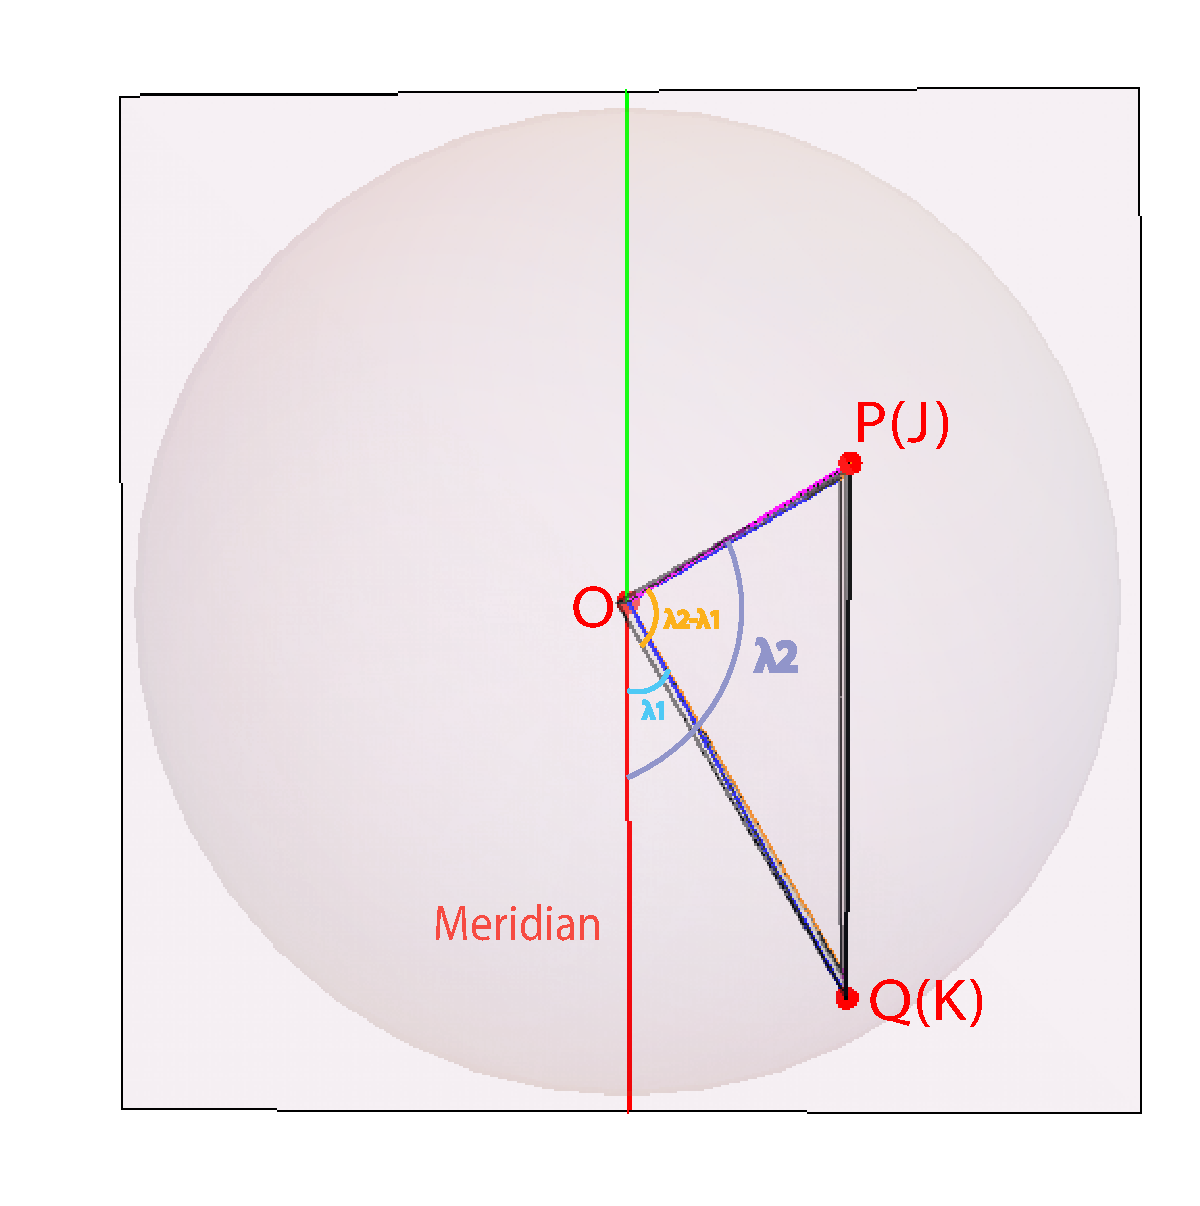
\includegraphics[width=5cm]{Visual1.pdf}
        \caption{Top View}
        \label{fig:great_circle_distance_visual_1}
    \end{minipage}
    \begin{minipage}[t]{0.275\textwidth}
        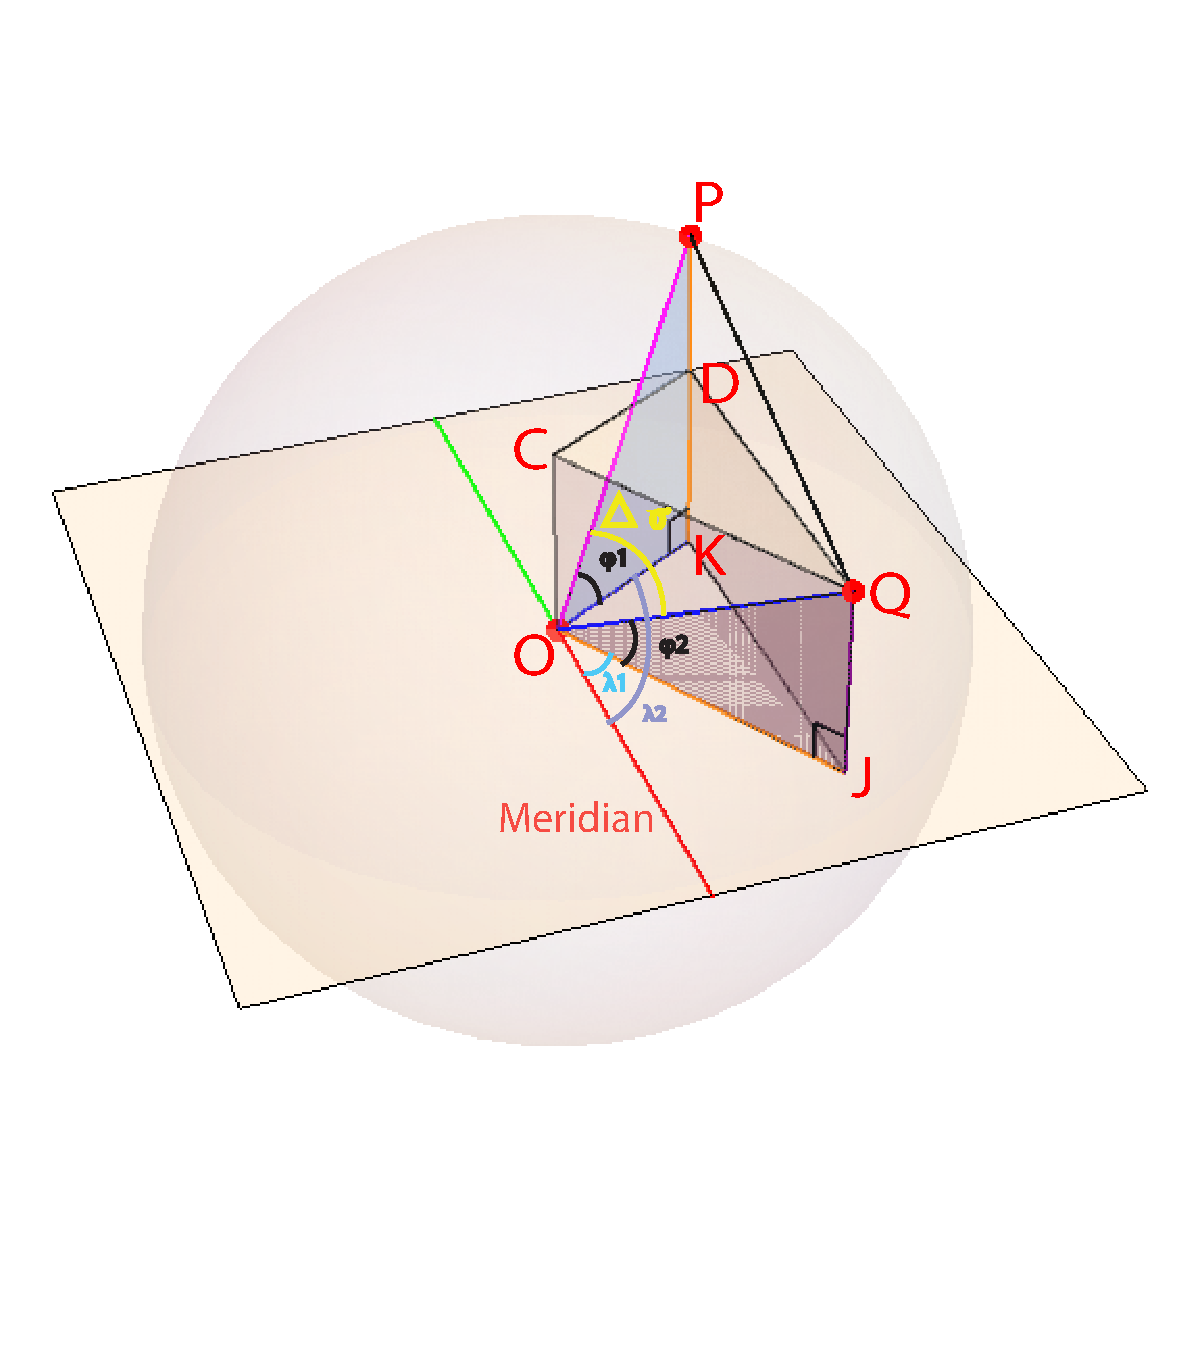
\includegraphics[width=5cm]{Visual2.pdf}
        \caption{Diagonal View}
        \label{fig:great_circle_distance_visual_2}
    \end{minipage}
    \begin{minipage}[t]{0.275\textwidth}
        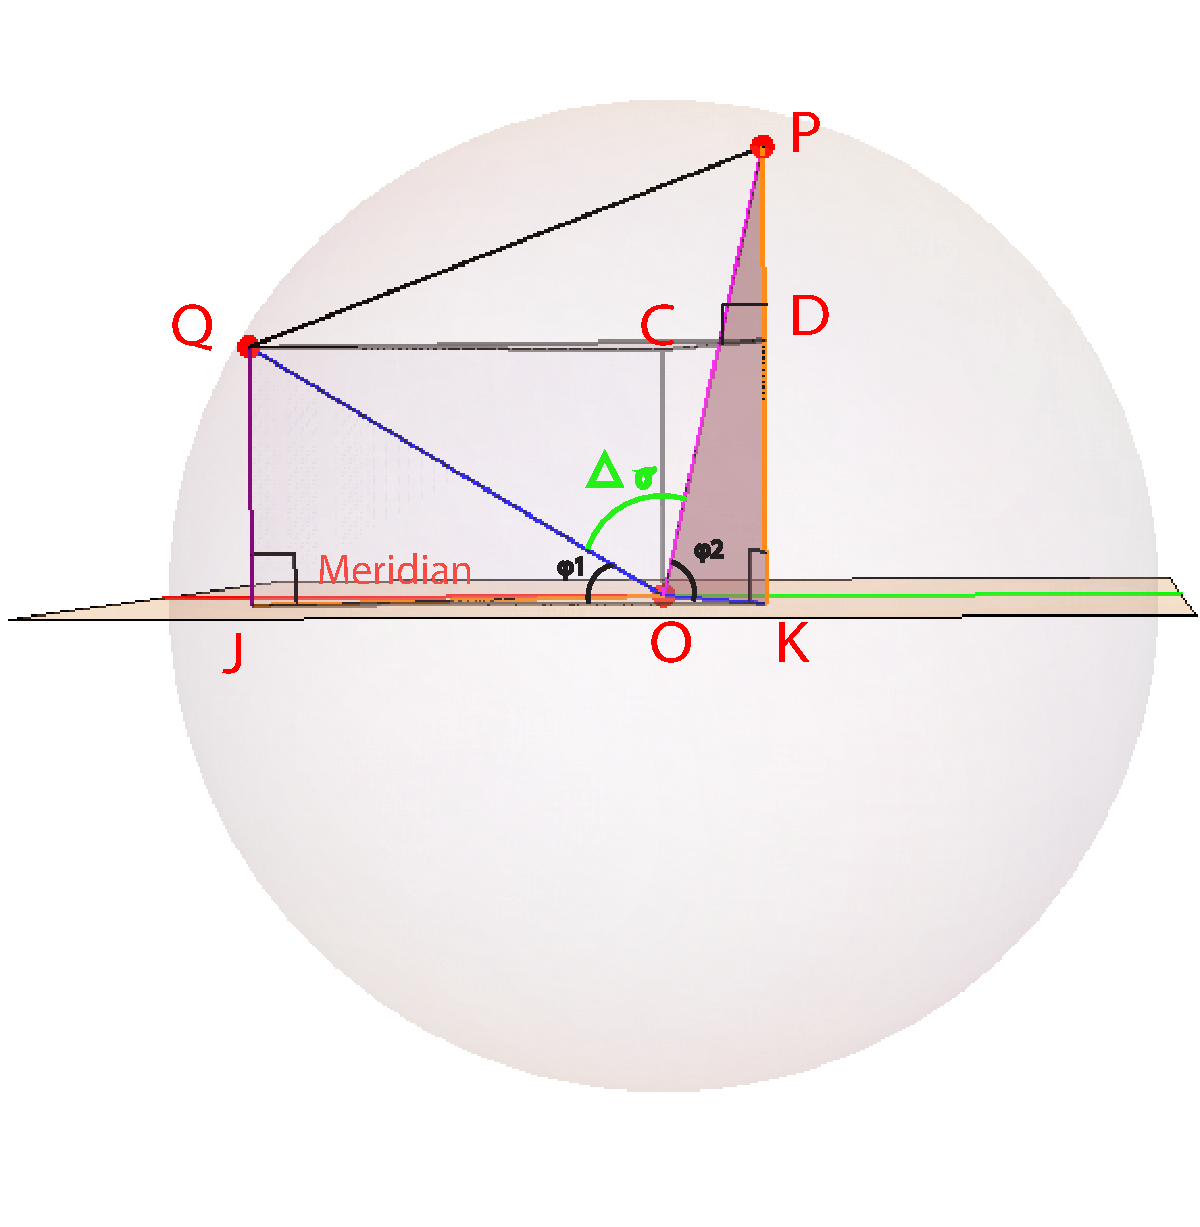
\includegraphics[width=5cm]{Visual3.pdf}
        \caption{Right View}
        \label{fig:great_circle_distance_visual_3}
    \end{minipage}
\end{figure}

\begin{gather}
\allowdisplaybreaks
\overline{OK}=\overline{OP}\cdot\cos\phi_1\\
\allowdisplaybreaks
\overline{OJ}=\overline{OQ}\cdot\cos\phi_2\\
\allowdisplaybreaks
\overline{JQ}=\overline{OQ}\cdot\sin\phi_2\\
\allowdisplaybreaks
\overline{PK}=\overline{OP}\cdot\sin\phi_2\\
\allowdisplaybreaks
\overline{QP}=2r\cdot\sin\left(\frac{\Delta\sigma}{2}\right)\\
\allowdisplaybreaks
\overline{QD}^2=\overline{DP}^2-\overline{QP}^2\\
\allowdisplaybreaks
\overline{QD}^2=\left(2r\cdot\sin\left(\frac{\Delta\sigma}{2}\right)\right)^2-\left(\overline{OP}\cdot\sin\phi_1-\overline{OQ}\cdot\sin\phi_2\right)^2\\
\overline{JK}=\overline{QD}\\ % 证明 三棱锥
\gamma=\lambda_1-\lambda_2\\
\overline{OP}=\overline{OQ}=r\\
2\,\overline{JO}\,\overline{KO}\cdot\cos\gamma=\overline{JO}^2+\overline{KO}^2-\overline{JK}^2\\
2\left(r\cdot\cos\phi_2\right)\left(r\cdot\cos\phi_1\right)\cdot\cos\gamma=\left(r\cdot\cos\phi_2\right)^2+\left(r\cdot\cos\phi_1\right)^2-\left(\left(2r\cdot\sin\left(\frac{\Delta\sigma}{2}\right)\right)^2-\left(r\cdot\sin\phi_1-r\cdot\sin\phi_2\right)^2\right)\\
2r^2\cdot\cos\phi_2\cos\phi_1\cos(\lambda_1-\lambda_2)=r^2\cos^2\phi_2+r^2\cos^2\phi_1-\left(4r^2\sin^2\left(\frac{\Delta\sigma}{2}\right)-\left(r^2\sin^2\phi_1+r^2\sin^2\phi_2-2r^2\sin\phi_1\sin\phi_2\right)\right)\\
\allowdisplaybreaks
2r^2\cos\phi_2\cos\phi_1\cos(\lambda_1-\lambda_2)=r^2\cos^2\phi_2+r^2\cos^2\phi_1-4r^2\sin^2\left(\frac{\Delta\sigma}{2}\right)+r^2\sin^2\phi_1+r^2\sin^2\phi_2-2r^2\sin\phi_1\sin\phi_2\\
\allowdisplaybreaks
r^2\left(2\cos\phi_2\cos\phi_1\cos\left(\lambda_1-\lambda_2\right)\right)=r^2\left(\cos^2\phi_2+\cos^2\phi_1-4\sin^2\left(\frac{\Delta\sigma}{2}\right)+\sin^2\phi_1+\sin^2\phi_2-2\sin\phi_1\sin\phi_2\right)\\
\allowdisplaybreaks
2\cos\phi_2\cos\phi_1\cos(\lambda_1-\lambda_2)=\cos^2\phi_2+\cos^2\phi_1-4\sin^2\left(\frac{\Delta\sigma}{2}\right)+\sin^2\phi_1+\sin^2\phi_2-2\sin\phi_1\sin\phi_2\\
\allowdisplaybreaks
4\sin^2\left(\frac{\Delta\sigma}{2}\right)=\cos^2\phi_2+\cos^2\phi_1+\sin^2\phi_1+\sin^2\phi_2-2\sin\phi_1\sin\phi_2-2\cos\phi_2\cos\phi_1\cos(\lambda_1-\lambda_2)\\
\allowdisplaybreaks
4\sin^2\left(\frac{\Delta\sigma}{2}\right)=2-2\sin\phi_1\sin\phi_2-2\cos\phi_2\cos\phi_1\cos(\lambda_1-\lambda_2)\\
\allowdisplaybreaks
\Delta\sigma=2\cdot\arcsin\left(\frac{\sqrt{2-2\sin\phi_1\sin\phi_2-2\cos\phi_2\cos\phi_1\cos(\lambda_1-\lambda_2)}}{2}\right)\\
\allowdisplaybreaks
\bigfrown{QP}=r\cdot\Delta\sigma\\
\allowdisplaybreaks
\bigfrown{QP}=2r\cdot\arcsin\left(\frac{\sqrt{2-2\sin\phi_1\sin\phi_2-2\cos\phi_2\cos\phi_1\cos(\lambda_1-\lambda_2)}}{2}\right)
\end{gather}

\section{Distance Program}

The part of the code which is covered with the red label \textbf{Gaode Map LBS API Key"} is where to put the API Key of the LBS, and it can be acquired for free at \href{http://lbs.amap.com/dev}{http://lbs.amap.com/dev}.

%%%%%%%%%%%%%%%%%%%%%%%%%%%%%%%%%%%%%%%%%%%%%%%%
\begin{mmaCell}[moredefined={candidate, demand}]{Code}
  candidate:={
    {1284.405914,463.870296},{1162.705645,593.059812},
    {1158.024866,418.934812},{857.518817,562.166667},
    {772.328629,343.106183},{725.520833,302.851478},
    {574.799731,448.891801},{464.333333,377.743952},
    {205.954301,315.021505},{920.241263,427.360215}
  };

  demand:={
    {1268.491263,453.572581},{1222.619624,427.360215},
    {1345.256048,492.891129},{1151.471774,429.232527},
    {1265.682796,527.528898},{1207.641129,589.315188},
    {1167.386425,630.506048},{1166.450269,582.762097},
    {1142.110215,528.465054},{1045.686156,503.188844},
    {1087.813172,597.740591},{948.325941,605.229839},
    {831.306452,426.424059},{816.327957,350.59543},
    {927.730511,382.424731},{823.817204,493.827285},
    {816.327957,584.634409},{689.946909,444.211022},
    {760.158602,241.065188},{678.713038,271.958333},
    {567.310484,409.573253},{568.24664,333.744624},
    {529.864247,461.997984},{420.334005,459.189516},
    {191.911962,335.616935},{240.59207,211.108199},
    {400.674731,204.555108},{541.098118,235.448253},
    {596.331317,482.593414},{695.563844,501.316532}
  };
\end{mmaCell}

\begin{mmaCell}[morepattern={r_, r, deg_, deg, x_, y_, p1_, p2_, p1, p2},moredefined={deg2rad, re, f, earthDistance, gaodeMapDistance, reqstr, req, resp, ToAssociations, res, UnitConvert, Entity, EntityProperty, QuantityMagnitude, URLExecute}]{Input}
  ClearAll[\mmaDef{\(\pmb{\phi}\)}]
  \mmaDef{\(\pmb{\phi}\)}[r_,\{\mmaPat{\(\pmb{\lambda}\)1_},\mmaPat{\(\pmb{\phi}\)1_}\},\{\mmaPat{\(\pmb{\lambda}\)2_},\mmaPat{\(\pmb{\phi}\)2_}\}]:=
    2r ArcSin[\mmaFrac{Sqrt[2-2Sin[\mmaPat{\(\pmb{\phi}\)1}]Sin[\mmaPat{\(\pmb{\phi}\)2}]-2Cos[\mmaPat{\(\pmb{\phi}\)1}]Cos[\mmaPat{\(\pmb{\phi}\)2}]Cos[\mmaPat{\(\pmb{\lambda}\)1}-\mmaPat{\(\pmb{\lambda}\)2}]]}{2}];
      0\(\pmb{\leq}\)\mmaPat{\(\pmb{\lambda}\)2}\(\pmb{\leq}\)\mmaPat{\(\pmb{\lambda}\)1}\(\pmb{\leq}\)\mmaDef{\(\pmb{\pi}\)};
  \mmaDef{\(\pmb{\phi}\)}[r_,\{\mmaPat{\(\pmb{\lambda}\)1_},\mmaPat{\(\pmb{\phi}\)1_}\},\{\mmaPat{\(\pmb{\lambda}\)2_},\mmaPat{\(\pmb{\phi}\)2_}\}]:=
    With[\{\mmaLoc{\(\pmb{\delta}\)}=-\mmaPat{\(\pmb{\lambda}\)2}\},\mmaDef{\(\pmb{\phi}\)}[r,\{\mmaPat{\(\pmb{\lambda}\)1}+\mmaLoc{\(\pmb{\delta}\)},\mmaPat{\(\pmb{\phi}\)1}\},\{0,\mmaPat{\(\pmb{\phi}\)2}\}]]/;
      \mmaPat{\(\pmb{\lambda}\)2}\(\pmb{\leq}\)\mmaPat{\(\pmb{\lambda}\)1}&&\mmaPat{\(\pmb{\lambda}\)2}<0;
  \mmaDef{\(\pmb{\phi}\)}[r_,\{\mmaPat{\(\pmb{\lambda}\)1_},\mmaPat{\(\pmb{\phi}\)1_}\},\{\mmaPat{\(\pmb{\lambda}\)2_},\mmaPat{\(\pmb{\phi}\)2_}\}]:=
    With[\{\mmaLoc{\(\pmb{\delta}\)}=\mmaPat{\(\pmb{\lambda}\)1}-\mmaDef{\(\pmb{\pi}\)}\},\mmaDef{\(\pmb{\phi}\)}[r,\{\mmaPat{\(\pmb{\lambda}\)1}-2\mmaLoc{\(\pmb{\delta}\)},\mmaPat{\(\pmb{\phi}\)1}\},\{\mmaPat{\(\pmb{\lambda}\)2},\mmaPat{\(\pmb{\phi}\)2}\}]]/;
      \mmaPat{\(\pmb{\lambda}\)2}\(\pmb{\leq}\)\mmaPat{\(\pmb{\lambda}\)1}&&\mmaPat{\(\pmb{\lambda}\)2}>0&&\mmaDef{\(\pmb{\pi}\)}<\mmaPat{\(\pmb{\lambda}\)1};
  \mmaDef{\(\pmb{\phi}\)}[r_,\{\mmaPat{\(\pmb{\lambda}\)1_},\mmaPat{\(\pmb{\phi}\)1_}\},\{\mmaPat{\(\pmb{\lambda}\)2_},\mmaPat{\(\pmb{\phi}\)2_}\}]:=
    \mmaDef{\(\pmb{\phi}\)}[r,\{\mmaPat{\(\pmb{\lambda}\)2},\mmaPat{\(\pmb{\phi}\)1}\},\{\mmaPat{\(\pmb{\lambda}\)1},\mmaPat{\(\pmb{\phi}\)2}\}]/;
      \mmaPat{\(\pmb{\lambda}\)1}<\mmaPat{\(\pmb{\lambda}\)2};
  deg2rad[deg_]:=\mmaFrac{deg \mmaDef{\(\pmb{\pi}\)}}{180};
  
  re=UnitConvert[
    Entity["Planet", "Earth"]
      [EntityProperty["Planet", "Radius"]], "Kilometers"]//
    QuantityMagnitude;
  f:=y==k x+b;
  Solve[\{
      f/.<|x\(\pmb{\to}\)1268.491263,y\(\pmb{\to}\)104.0745339802915|>,
      f/.<|x\(\pmb{\to}\)1142.110215,y\(\pmb{\to}\)104.0570672802915|>
    \},\{\mmaFnc{k},\mmaFnc{b}\}];
  Solve[\{
      f/.<|x\(\pmb{\to}\)453.572581,y\(\pmb{\to}\)30.6690810197085|>,
      f/.<|x\(\pmb{\to}\)528.465054,y\(\pmb{\to}\)30.6592861197085|>
    \},\{\mmaFnc{k},\mmaFnc{b}\}];
  \mmaDef{k\(\pmb{\lambda}\)}=k/.%%[[1]];
  \mmaDef{b\(\pmb{\lambda}\)}=b/.%%%[[1]];
  \mmaDef{k\(\pmb{\phi}\)}=k/.%%%[[1]];
  \mmaDef{b\(\pmb{\phi}\)}=b/.%%%%[[1]];
  \mmaDef{\(\pmb{\xi}\)}[\{x_,y_\}]:=\{\mmaDef{k\(\pmb{\lambda}\)} \mmaPat{x}+\mmaDef{b\(\pmb{\lambda}\)},\mmaDef{k\(\pmb{\phi}\)} \mmaPat{y}+\mmaDef{b\(\pmb{\phi}\)}\};
  earthDistance[p1_,p2_]:=\mmaDef{\(\pmb{\phi}\)}[re,deg2rad/@\mmaDef{\(\pmb{\xi}\)}@p1,deg2rad/@\mmaDef{\(\pmb{\xi}\)}@p2];

  gaodeMapDistance[p1_,p2_]:=Module[\{\},
    reqstr:="http://restapi.amap.com/v3/distance";
    req[\{\mmaPat{\(\pmb{\lambda}\)1_},\mmaPat{\(\pmb{\phi}\)1_}\},\{\mmaPat{\(\pmb{\lambda}\)2_},\mmaPat{\(\pmb{\phi}\)2_}\}]:=URLExecute[reqstr,\{
      "key"\(\pmb{\to}\)"\mmaFmt{Gaode Map LBS API Key}",
      "origins"\(\pmb{\to}\)ToString[\mmaPat{\(\pmb{\lambda}\)1}]<>","<>ToString[\mmaPat{\(\pmb{\phi}\)1}],
      "destination"\(\pmb{\to}\)ToString[\mmaPat{\(\pmb{\lambda}\)2}]<>","<>ToString[\mmaPat{\(\pmb{\phi}\)2}],
      "type"\(\pmb{\to}\)1,
      "output"\(\pmb{\to}\)"JSON"
    \},"JSON"];
    resp=ToAssociations[res=req[\mmaDef{\(\pmb{\xi}\)}[p1],\mmaDef{\(\pmb{\xi}\)}[p2]]];
    N[\{
      \mmaFrac{ToExpression[resp["results"][[1]]["distance"]]}{1000},
      ToExpression[resp["results"][[1]]["duration"]]
    \}]
  ];
\end{mmaCell}

\begin{mmaCell}[moredefined={distanceMap, demand, candidate, gaodeMapDistance, earthDistance},morelocal={map, i, j, dis, d}]{Input}
  distanceMap=Module[\{map=\{\},i,j,dis,d\},
    For[i=1,i\(\pmb{\leq}\)Length[demand],i++,
      For[j=1,j\(\pmb{\leq}\)Length[candidate],j++,
        dis=gaodeMapDistance[demand[[i]],candidate[[j]]];
        d=\{
          i,FromCharacterCode[64+j],
          demand[[i]],candidate[[j]],
          \mmaDef{\(\pmb{\xi}\)}[demand[[i]]],\mmaDef{\(\pmb{\xi}\)}[candidate[[j]]],
          earthDistance[demand[[i]],candidate[[j]]],
          dis[[1]],dis[[2]]
        \};
        AppendTo[map,d];
      ];
    ];
    map
  ];
  Grid[Prepend[distanceMap,\{
    "DP","CP","DP Mercator","CP Mercator",
    "DP L-L","CP L-L","Great-Circle","Driving","Duration"
  \}],Frame\(\pmb{\to}\)All]
\end{mmaCell}
%%%%%%%%%%%%%%%%%%%%%%%%%%%%%%%%%%%%%%%%%%%%%%%%

\section{Computational Details}
\begin{minted}{swift}
import Foundation

// Constants
let selectionBias: Double = log(2) / log(1.1)

let locationArray = [
    [1268.491263, 453.572581, 33],
    [1222.619624, 427.360215, 35],
    [1345.256048, 492.891129, 22],
    [1151.471774, 429.232527, 29],
    [1265.682796, 527.528898, 28],
    [1207.641129, 589.315188, 34],
    [1167.386425, 630.506048, 37],
    [1166.450269, 582.762097, 45],
    [1142.110215, 528.465054, 37],
    [1045.686156, 503.188844, 45],
    [1087.813172, 597.740591, 50],
    [948.325941, 605.229839, 33],
    [831.306452, 426.424059, 29],
    [816.327957, 350.59543, 35],
    [927.730511, 382.424731, 43],
    [823.817204, 493.827285, 42],
    [816.327957, 584.634409, 23],
    [689.946909, 444.211022, 34],
    [760.158602, 241.065188, 31],
    [678.713038, 271.958333, 37],
    [567.310484, 409.573253, 41],
    [568.24664, 333.744624, 24],
    [529.864247, 461.997984, 29],
    [420.334005, 459.189516, 32],
    [191.911962, 335.616935, 32],
    [240.59207, 211.108199, 22],
    [400.674731, 204.555108, 24],
    [541.098118, 235.448253, 26],
    [596.331317, 482.593414, 33],
    [695.563844, 501.316532, 31]
]


let candidateCoordinates = [
    [1284.405914, 463.870296],
    [1162.705645, 593.059812],
    [1158.024866, 418.934812],
    [857.518817, 562.166667],
    [772.328629, 343.106183],
    [725.520833, 302.851478],
    [574.799731, 448.891801],
    [464.333333, 377.743952],
    [205.954301, 315.021505],
    [920.241263, 427.360215]
]

let dMap = [[0.323, 4.148, 2.856, 8.355, 7.896, 9.622, 13.435, 13.093, 18.88, 7.307],
[1.027, 2.922, 1.404, 7.31, 7.255, 8.981, 12.029, 11.691, 17.835, 5.98],
[1.129, 4.25, 3.678, 8.185, 8.819, 10.545, 13.261, 12.923, 18.71, 7.137],
[2.277, 3.266, 0.186, 6.094, 6.125, 7.851, 10.899, 10.561, 16.619, 4.85],
[2.065, 2.335, 2.868, 7.138, 8.426, 10.152, 12.214, 11.876, 17.663, 6.09],
[3.453, 1.318, 3.802, 5.635, 9.212, 10.814, 11.644, 12.156, 16.16, 6.37],
[4.521, 1.17, 3.894, 4.997, 8.734, 10.761, 11.166, 11.678, 15.682, 5.892],
[3.374, 0.571, 2.547, 5.067, 7.656, 9.559, 10.892, 10.554, 15.592, 4.768],
[3.073, 1.217, 2.246, 5.529, 7.369, 9.258, 10.605, 10.267, 16.054, 4.481],
[4.516, 3.019, 3.054, 4.898, 5.574, 8.083, 8.81, 8.472, 14.113, 2.686],
[4.966, 1.851, 3.436, 3.474, 7.281, 10.303, 10.224, 11.22, 14.74, 5.434],
[6.417, 3.302, 4.887, 1.706, 5.582, 9.352, 8.525, 8.879, 13.041, 3.889],
[7.632, 6.135, 6.17, 3.84, 2.041, 5.771, 5.452, 5.114, 10.802, 1.52],
[7.778, 8.145, 6.248, 5.526, 1.434, 4.177, 6.416, 6.078, 11.693, 2.994],
[5.51, 5.877, 3.98, 4.395, 2.747, 5.217, 7.611, 7.273, 12.877, 1.607],
[8.158, 5.043, 6.628, 2.792, 4.274, 8.004, 6.706, 7.06, 11.222, 2.624],
[7.877, 4.762, 6.347, 0.849, 4.554, 10.47, 7.058, 7.412, 11.574, 3.842],
[9.385, 7.249, 7.923, 4.356, 2.323, 5.89, 4.033, 4.387, 8.549, 3.664],
[8.295, 8.662, 6.765, 10.48, 2.659, 1.881, 6.795, 6.915, 11.863, 4.755],
[12.784, 11.287, 11.322, 9.51, 3.5, 0.968, 5.825, 6.002, 10.95, 6.993],
[12.198, 10.701, 10.736, 7.762, 5.441, 7.449, 1.965, 1.627, 7.197, 6.407],
[13.287, 12.194, 11.757, 9.126, 6.312, 6.201, 2.901, 3.12, 8.655, 7.82],
[12.181, 9.066, 10.651, 6.133, 4.914, 8.247, 1.052, 2.559, 6.721, 6.647],
[13.369, 10.458, 12.043, 7.525, 6.306, 9.639, 2.444, 2.065, 4.841, 8.039],
[17.785, 14.804, 16.323, 11.871, 10.652, 13.036, 6.79, 6.199, 1.043, 12.385],
[17.008, 17.375, 15.478, 13.165, 11.973, 10.429, 7.368, 6.015, 5.152, 13.719],
[14.554, 13.057, 13.092, 10.204, 7.302, 9.975, 6.217, 4.676, 9.567, 8.81],
[12.294, 10.797, 10.832, 7.944, 5.042, 7.715, 3.957, 4.176, 9.711, 6.55],
[12.352, 10.273, 10.89, 6.36, 5.595, 7.603, 0.795, 3.063, 7.225, 6.561],
[10.154, 7.039, 8.624, 3.668, 3.03, 6.699, 4.504, 4.858, 9.02, 4.62]]

let costs = [650, 530, 400, 350]
let capacity = [350, 250, 110, 70]

func d(_ location: Int, _ candidate: Int) -> Double {
    return dMap[location-1][candidate-1]
}

// Returns distance between a demand point and a candidate point
func distanceArray(location: Int, candidates: [Int]) -> (array: [Double], sum: Double) {
    var distanceArray = [Double]()
    var sum = 0.0
    
    for i in 0..<candidates.count {
        distanceArray.append(d(location, candidates[i]))
        sum += pow(distanceArray[i], -selectionBias)
    }
    
    return (distanceArray, sum)
}

// Probability of an EV user at a demand point going to each of the available candidate positions
func probabilityArray(location: Int, candidates: [Int]) -> [Double] {
    let dArray = distanceArray(location: location, candidates: candidates)
    
    var probabilityArray = [Double]()
    
    for i in 0..<candidates.count {
        probabilityArray.append(pow(dArray.array[i], -selectionBias)
        / dArray.sum * locationArray[location-1][2])
    }
    return probabilityArray
}

// Number of EVs going to each of the specified locations per day
func totalDemand(candidates: [Int]) -> [Double] {
    var demandPerCandidate = Array<Double>(repeating: 0, count: candidates.count)
    for l in 1...locationArray.count {
        let cprobArray = probabilityArray(location: l, candidates: candidates)
        for c in 0..<cprobArray.count {
            demandPerCandidate[c] += cprobArray[c]
        }
    }
    return demandPerCandidate
}

// Total initial and construction cost
func totalCost(candidates: [Int]) -> (C: Double, b: Double, c_dist: [Int: Double])? {
    let td = totalDemand(candidates: candidates)
    
    var constructionCost = 0.0
    
    for i in td {
        if i > 350 {return nil}
        else if i > 250 {
            constructionCost += 6500000
        } else if i > 110 {
            constructionCost += 5300000
        } else if i > 70 {
            constructionCost += 4000000
        } else {
            constructionCost += 3500000
        }
    }
    
    var consumerCost = 0.0
    
    var distanceByCandidate = [Int: Double]()
    
    for l in 1...locationArray.count {
        var Ed = 0.0
        let dA = distanceArray(location: l, candidates: candidates).array
        let pA = probabilityArray(location: l, candidates: candidates)
        for i in 0..<dA.count {
            Ed += dA[i] * pA[i]
            distanceByCandidate[candidates[i]] = distanceByCandidate[candidates[i]] == nil ?
            dA[i] * pA[i] : distanceByCandidate[candidates[i]]! + dA[i] * pA[i]
        }
        consumerCost += Ed
    }
    
    return (consumerCost, constructionCost, distanceByCandidate)
    
}

func findOptimalCandidates(n: Int) -> (c_cost: Double, b_cost: Double, candidates: [Int]) {
    var optimalCandidates = [Int]()
    var optimalDailyCost = 0.0
    var optimalConstructionCost = 0.0
    for i in 1...10 {
        var jArray = Array(1...10)
        jArray.remove(at: i-1)
        for j in jArray {
            var kArray = jArray
            kArray.remove(at: kArray.index(of: j)!)
            for k in kArray {
                var lArray = kArray
                lArray.remove(at: lArray.index(of: k)!)
                for l in lArray {
                    if let t = totalCost(candidates: [i,j,k,l]) {
                        if optimalConstructionCost > 0 && t.b < optimalConstructionCost {
                            optimalDailyCost = t.C
                            optimalCandidates = [i,j,k,l]
                            optimalConstructionCost = t.b
                        } else if optimalDailyCost == 0 {
                            optimalDailyCost = t.C
                            optimalConstructionCost = t.b
                        }
                    }
                }
            }
        }
    }
    
    return (optimalDailyCost, optimalConstructionCost, optimalCandidates)
}
\end{minted}

\section{Additional Resources}
Due to the limitation of the competition, it is clear that we cannot show all of our progress in completing this research, and we decided to put most of our selected work online publicly for access.

If you wish, please download the programs and raw files from \href{http://tenic.xyz/IMMC2018}{https://tenic.xyz/IMMC2018}.

\newpage
\begin{thebibliography}{9}
\bibitem{Uniform behavior} 
N. Rotering and M. Ilic, “Optimal charge control of plug-in hybrid electric vehicles in deregulated electricity markets,”
\textit{IEEE Transactions on Power Systems}, vol. 26, pp. 1021–1029, 2011.
\bibitem{EV sales}
“China Plug-in Sales for 2017-Q4 and Full Year – Update.” EV-Volumes - The Electric Vehicle World Sales Database, EV Volumes, www.ev-volumes.com/country/china/. 
 
\bibitem{Incentives} 
P. Richardson, D. Flynn, and A. Keane, “Optimal charging of electric vehicles in low-voltage distribution systems,” \textit{IEEE Transactions on Power Systems}, vol. 27, pp. 268–279, 2012. 

\bibitem{Charging a Capacitor}
 “Charging a Capacitor: Solutions.” Microsoft Word - workshop 06 charging a capacitor solutions.Doc, Massachusetts Institute of Technology Department of Physics, web.mit.edu/molly/Public/circuits-b.pdf. 

\bibitem{Constraints}
Equality and Inequality Constraints, mat.gsia.cmu.edu/classes/QUANT/NOTES/chap4/node6.html. 

\bibitem{queueing system}
Bolch, G.; Greiner, S.; de Meer, H.; Trivedi, K. S. (1998). "Single Station Queueing Systems". \textit{Queueing Networks and Markov Chains.} pp. 209–262. doi:10.1002/0471200581.ch6. ISBN 0471193666.

\bibitem{q}
Teknomo, Kardi. “M/M/s/N Queuing System.” \textit{Queuing Theory Tutorial - M/M/s/N Queuing System.} Evoledu, people.revoledu.com/kardi/tutorial/Queuing/MMsN-Queuing-System.html.
\bibitem{n}
Belk, Jim. “Linear Algebra with ODEs.” \textit{Math 213}, 5 Feb. 2018, New York, Campus Road, faculty.bard.edu/belk/math213/.
\end{thebibliography}

\end{document}